\documentclass[12pt]{ucsddissertation}
% mathptmx is a Times Roman look-alike (don't use the times package)
% It isn't clear if Times is required. The OGS manual lists several
% "standard fonts" but never says they need to be used.
\usepackage{mathptmx}
\usepackage[NoDate]{currvita}
\usepackage{array}
\usepackage{tabularx}
\usepackage{booktabs}
\usepackage{ragged2e}
\usepackage{microtype}
\usepackage[breaklinks=true,pdfborder={0 0 0}]{hyperref}
\usepackage{graphicx}
\AtBeginDocument{%
	\settowidth\cvlabelwidth{\cvlabelfont 0000--0000}%
}

% OGS recommends increasing the margins slightly.
\increasemargins{.1in}

% These are just for testing/examples, delete them
\usepackage{trace}
%\usepackage{showframe} % This package was just to see page margins
\usepackage[english]{babel}
\overfullrule5pt
% ---

% Packages specific to this dissertation
\usepackage{amsmath}
\usepackage{amssymb}
\usepackage{contour}
%\usepackage{amsthm}
\usepackage{xcolor}
\usepackage{bussproofs}
\usepackage{listings}
\usepackage{hyperref}
\usepackage{tabularx}
\usepackage{tikz}
\usepackage{macros}
\usepackage{xspace}
\usepackage{adjustbox}
%\usepackage{gensymb}
%\usepackage{pgfplots}
\usepackage{etex}
\usepackage{todonotes}
\usepackage{mfirstuc}
\usepackage{changebar}
\usepackage{subcaption}
\usepackage{enumitem}

\usetikzlibrary{calc}
\usetikzlibrary{backgrounds}
\usetikzlibrary{patterns}
\usetikzlibrary{decorations}
\usetikzlibrary{arrows}
\usetikzlibrary{decorations.markings}
\usetikzlibrary{positioning}

\newtheorem{theorem}{Theorem}
\newtheorem{lemma}{Lemma}
\newtheorem{definition}{Definition}

% Required information
\title{Verification of Sampled-Data Systems using Coq}
\author{Daniel Ricketts}
\degree{Computer Science}{Doctor of Philosophy}
% Each member of the committee should be listed as Professor Foo Bar.
% If Professor is not the correct title for one, then titles should be
% omitted entirely.
\chair{Professor Sorin Lerner}
% Your committee members (other than the chairs) must be in alphabetical order
\committee{Professor Samuel Buss}
\committee{Professor William Griswold}
\committee{Professor Ranjit Jhala}
\committee{Professor Todd Millstein}
\degreeyear{2017}

% Start the document
\begin{document}
% Begin with frontmatter and so forth
\frontmatter
\maketitle
\makecopyright
\makesignature
% Optional
\begin{dedication}
\setsinglespacing
\raggedright % It would be better to use \RaggedRight from ragged2e
\parindent0pt\parskip\baselineskip
In recognition of reading this manual before beginning to format the
doctoral dissertation or master's thesis; for following the
instructions written herein; for consulting with OGS Academic Affairs
Advisers; and for not relying on other completed manuscripts, this
manual is dedicated to all graduate students about to complete the
doctoral dissertation or master's thesis.

In recognition that this is my one chance to use whichever
justification, spacing, writing style, text size, and/or textfont that
I want to while still keeping my headings and margins consistent.
\end{dedication}
% Optional
\begin{epigraph}
\vskip0pt plus.5fil
\setsinglespacing
{\flushright
True ease in writing comes from art, not chance,\\
As those move easiest who have learn'd to dance.\\
'T is not enough to no harshness gives offence,---\\
The sound must seem an echo to the sense.

\vskip\baselineskip
\textit{Alexander Pope}\par}
\vfil
\begin{center}
You write with ease to show your breeding,\\
But easy writing's curst hard reading.

\vskip\baselineskip
\textit{Richard Brinsley Sheridan}
\end{center}
\vfil
\noindent Writing, at its best, is a lonely life. Organizations for
writers palliate the writer's loneliness, but I doubt if they improve
his writing. He grows in public stature as he sheds his loneliness and
often his work deteriorates. For he does his work alone and if he is a
good enough writer he must face eternity, or the lack of it, each day.

\vskip\baselineskip
\hskip0pt plus1fil\textit{Ernest Hemingway}\hskip0pt plus4fil\null

\vfil
\end{epigraph}

% Next comes the table of contents, list of figures, list of tables,
% etc. If you have code listings, you can use \listoflistings (or
% \lstlistoflistings) to have it be produced here as well. Same with
% \listofalgorithms.
\tableofcontents
\listoffigures
\listoftables

% Preface
\begin{preface}
Almost nothing is said in the manual about the preface. There is no
indication about how it is to be typeset. Given that, one is forced to
simply typeset it and hope it is accepted. It is, however, optional
and may be omitted.
\end{preface}

% Your fancy acks here. Keep in mind you need to ack each paper you
% use. See the examples here. In addition, each chapter ack needs to
% be repeated at the end of the relevant chapter.
\begin{acknowledgements}
I would like to acknowledge Professor Eta Theta for his support as the
chair of my committee. Through multiple drafts and many long nights,
his guidance has proved to be invaluable.

I would also like to acknowledge the ``Smith Clan'' of lab~28, without
whom my research would have no doubt taken fives times as long. It is
their support that helped me in an immeasureable way.

Chapter 2, in full, is a reprint of the material as it appears in
Numerical Grid Generational in Computational Fluid Mechanics~2009.
Smith, Laura; Smith, Jane~D., Pineridge Press,~2009. The dissertation
author was the primary investigator and author of this paper.

Chapter 3, in part, has been submitted for publication of the material
as it may appear in Education Mechanics,~2009, Smith, Laura; Smith,
Jane~D., Trailor Press,~2009. The dissertation author was the primary
investigator and author of this paper.

Chapter 5, in part is currently being prepared for submission for
publication of the material. Smith, Laura; Smith, Jane~D\@. The
dissertation author was the primary investigator and author of this
material.
\end{acknowledgements}

% Stupid vita goes next
\begin{vita}
\noindent
\begin{cv}{}
\begin{cvlist}{}
\item[1996] Bachelor of Arts, University of California, Berkeley
\item[1996--2000] U.S. Marines
\item[2000--2002] Teaching Assistant, Department of Mechanical
Engineering\\University of California, San Diego
\item[2002--2006] Research Assistant, University of California, San
Diego
\item[2010] Doctor of Philosophy, University of California, San Diego
\end{cvlist}
\end{cv}

% This puts in the PUBLICATIONS header. Note that it appears inside
% the vita environment. It is optional.
\publications
\noindent``Distributions of Control Points in a System for Analysis of Stress
Distribution'' IRE Transactions of the I.R.E\@. Professional Group on
Automatic Control, vol. AC-7, pp 272--289, September 2005

% This puts in the FIELDS OF STUDY. Also inside vita and also
% optional.
\fieldsofstudy
\noindent Major Field: Engineering (Specialization or Focused Studies)
\vskip\baselineskip
Studies in Applied Mathematics\par
Professors Alpha Beta and Gamma Delta
\vskip\baselineskip
Studies in Mechanices\par
Professors Epsilon Zeta and Eta Theta
\vskip\baselineskip
Studies in Electromagnetism\par
Professors Iota Kappa and Lambda Mu
\end{vita}

% Put your maximum 350 word abstract here.
\begin{dissertationabstract}
The Abstract begins here. The abstract is limited to 350 words for a
doctoral dissertation. It should consist of a short statement of the
problem, a brief explanation of the methods and procedures employed in
generating the data, and a condensed summary of the findings of the
study. The abstract may continute onto a second page if necessary. The
text of the abstract must be double spaced.
\end{dissertationabstract}

% This is where the main body of your dissertation goes!
\mainmatter

% Optional Introduction
\begin{dissertationintroduction}
Errors in cyber-physical systems (CPS) can lead to disastrous consequences,
including loss of life.  These consequences mean that such systems demand
the most rigorous verification techniques.  There has been a variety of
work on developing fully-automated tools for verification of cyber-physical
systems~\cite{PHAVerSTTT08,HyTechCAV97}, but due to the complexity of the
domain, these tools are only able to verify particular classes of systems
and properties.  On the other hand, all cyber-physical systems are in range
for deductive verification in a proof assistant, at least in theory.  In
this technique, a user writes a formal model of a system in the language of
the proof assistant and then interactively proves it correct. However, one
of the typically-stated drawbacks of verification in proof assistants is
the extremely high manual labor cost required to produce these proofs.

Mitigating this manual proof burden requires powerful higher-order proof
rules that capture common proof strategies. Prior work in deductive
verification has approached this task by designing general-purpose,
complete proof calculi for hybrid systems~\cite{platzer???,HHL???}. Hybrid
systems are CPS models comprised of both a discrete component (e.g. control
software) and a continuous component (the physical world). While powerful,
the generality of the proof calculi prevents them from leveraging
particular common characteristics of cyber-physical systems. For example,
no proof rule in~\cite{platzer??} assumes that the time between executions
of a controller is bounded because this is not true of all hybrid
systems. However, this is true of many realistic hybrid systems, and proofs
about such systems will tend to follow a similar proof structure. Thus, it
is beneficial to complement general hybrid system proof rules with domain
specific proof rules that capture common reasoning patterns.

This dissertation presents and applies a series of proof rules that capture
common reasoning patterns in the important domain of \emph{periodic
  sampled-data systems}~\cite{chen1995sampled}. In such a system, there is
a digital controller that runs periodically. In between executions of the
controller, the system evolves according to continuous physical
dynamics. Many modern cyber-physical systems fit into this domain. The
remainder of the introduction provides an overview of the proof rules. In
general, the rules seek to leverage timing characteristics of systems and
improve modularity of reasoning.

In \textbf{Chapter~\ref{chap:memo15}} we present two rules: one for
verifying a single sampled-data component under assumption on the
environment and another for composing such a component with another that
satisfies this assumption. The first rule decomposes verification into a
property of the discrete controller and the continuous dynamics,
automatically handling the fact that the time between executions of the
controller is bounded. This tailored decomposition eliminates some of the
basic tedious manipulation common to every sampled-data system, allowing
one to focus on the application specific aspects of verification. The
second proof rule allows for component composition with non-cylical
assumptions -- that is, a component $C1$ can guarantee an invariant $Q$
while assuming and invariant $P$ guaranteed by $C2$. However, $C2$ cannot
rely on the invariance of $P$ when guaranteeing $Q$. In spite of this
restriction, we show that such a rule has important applications for
verifying controllers in the presence of sensor error and delay.

Next, \textbf{Chapter~\ref{chap:emsoft16}} presents a general framework for
building sampled-data systems \emph{modularly}. This framework differs from
the above composition approach by requiring that each component provide a
stronger interface. In particular, rather than proving invariance of a
property, each component provides preservation of an inductive invariant,
and a notion of progress of the system under that inductive invariant. This
stronger interface comes at a minor cost while proving two important
benefits. First, it allows for cyclic dependencies between sampled-data
components, thus removing the restriction from
Chapter~\ref{chap:memo15}. Second, it allows us to explore a richer set of
operators for modularly building and verifying sampled-data components,
namely substitution, conjunction, and disjunction. It is this second
benefit that we explore thoroughly by applying our framework to build
verified 3-dimensional geofences for a UAV. We show that our theory can
handle the important situation in which different components output to the
same set of actuators, as exemplified by the geofence application.

Finally, in \textbf{Chapter~\ref{chap:exp-smpl}}, we revisit verification
of a single sampled-data system component. Contrary to our prior
approaches, we began by building a geofence that was good enough to be
adopted by the popular open source UAV autopilot called
Ardupilot~\cite{???}. After building such a module (now available in the
latest Ardupilot release), we attempted to formally verify a component of
it in Coq, particularly the logic that prevents the vehicle from violating
a boundary in a single spatial dimension. Similar logic is present in the
atomic components from Chapters~\ref{chap:memo15} and~\ref{chap:emsoft16},
but realistic performance requirements for Ardupilot resulted in
considerably more complicated control logic. This additional complexity
demanded better proof rules, and we built rules that improve upon the state
of the art in formal verification in two ways.

First, deductive techniques typically involve some continuous analogue of
induction, e.g. differential induction~\cite{Ghorbal14diffinv} or barrier
certificates~\cite{prajna04barrier}. Recent work from the control theory
community~\cite{kong2013barrier,xu15barrier,nguyen16barrier} has produced a
new version of barrier certificates that are less conservative for closed
properties. We provide the first implementation of this approach in a
formal verification context, and demonstrate its ease of use on a component
of the ardupilot geofencing module.

Second, control systems are often designed under the assumption that
controllers run continuously, while the actual implementation is typically
a sampled-data system. System designers can compensate for this (and other)
approximations by adding a safety ``buffer'' to the system. For example,
the ardupilot geofence module stops the vehicle 1 meter prior to the actual
safety boundary. We developed a proof rule that formalizes this design
approach by decomposing verification into a condition on the continuous
time approximation and another on the approximation error.  This rule
allows one to perform the majority of reasoning in a purely continuous
model using powerful techniques resulting from over a century of control
theory research.

As already mentioned, our running application in this work is a geofencing
controller for UAVs, an important application due to their potential safety
thread combined with widespread use by hobbyists and businesses alike. We
would like to ensure that the controller we build and verify are not toy
models. We have attempted to justify the realistic nature of our work by
flying the controllers we verify on an actual quadcopter. Throughout this
dissertation, we discuss lessons learned from this experience.

Rigorous verification requires that results be mechanically checked in some
way. Rather than implementing a standalone tool for this task, we performed
all verification within the foundational Coq proof assistant. Previous
work~\cite{yang2011understanding-compiler-bugs} has empirically
demonstrated that foundationally verified systems are highly
reliable. While important, we would like to emphasize a less discussed
benefit of higher-order proof assistants like Coq. A standalone domain
specific verification tool would require adding each proof rule as an
axiom. Moreover, a new proof rule might have side conditions not
expressible in the tool's logic, requiring custom reasoning to handle these
side conditions. In this context, the axiom and associated custom reasoning
have the potential to compromise soundness.

On the other hand, the \emph{expressiveness} of Coq allows one add new
proof rules as theorems that are formally proven within Coq's logic. This
means that one can extend any given set of general proof rules in Coq
(e.g. general proof calculi for hybrid systems) with powerful domain
specific proof rules (e.g. our sampled-data system rules), without
compromising soundness. Such an extension improves verification
productivity by ensuring that a user can apply the right domain-specific
proof rule for his or her application while still being able to depend on
the above mentioned reliability guarantees. It is thus the view of the
dissertation author that the expressive framework of a higher-order proof
assistant is crucial to scaling formal verification to realistic
cyber-physical systems, and we hope that the proof rules and associated
applications in this document provide evidence for this claim.

\end{dissertationintroduction}

\chapter{Preliminaries}
\label{chap:prelim}
In this chapter, we describe the logical framework used in
Chapters~\ref{chap:memo15}
and~\ref{chap:emsoft16}. Chapter~\ref{chap:exp-smpl} uses a different
framework, so the logical background is presented within that chapter. All
of our work is formalized inside the Coq proof assistant, but for
exposition purposes, we focus on the mathematical concepts rather than
concrete Coq syntax.

\section{Linear Temporal Logic}
In Chapters~\ref{chap:memo15} and~\ref{chap:emsoft16}, we encode
sampled-data systems and their properties within discrete-time linear
temporal logic (LTL).  An LTL formula specifies the possible traces of a
system.  In our model, a trace is an infinite sequence of states
representing observations of a system at discrete points in time.  A state
is a mapping from variables to real numbers.  Inspired by Lamport's
Temporal Logic of Actions (TLA)~\cite{lamport1994temporal}, formulas in our
logic are classified into \emph{state formulas} (predicates over a single
state), \emph{action formulas} (state relations specifying system
transitions), and \emph{trace formulas} (predicates over traces).  In
action formulas, the values of variables in the current state are notated
using bold script, e.g. \tlavar{x}, while the values of variables in the
next state use bold script with a prime, e.g. \tlanextvar{x}.  Variables
not mentioned in a formula are unconstrained.

For example, the following formula describes a system where the initial
value of \tlavar{x} is 0 and the value of \tlavar{x} is incremented during
each transition.
\[
\tlavar{x} = 0~\wedge~\Always\left(\tlanextvar{x} = \tlavar{x} + 1\right)
\]
The initial condition ($\tlavar{x} = 0$) is a state formula.  The
transition relation ($\tlanextvar{x} = \tlavar{x} + 1$) is an action
formula and refers to values in the next state using a prime,
e.g. \tlanextvar{x}.  Both the transition relation and the property are
lifted to trace formulas using the always modality ($\Box$).  When always
is applied to an action formula, it means that all pairs of temporally
adjacent states are related by the action formula.  When always is applied
to a state formula, it means that all states satisfy the property.

Finally, the semantics of formulas is defined in terms of two relations:
``models'' (written $tr \models P$) states when a predicate ($P$) holds on
a trace ($tr$), and ``entails'' (written $P \entails Q$, or just $\entails
Q$ when $P$ is trivial) states when one predicate implies another on
\emph{all} traces, i.e.
\begin{definition}[LTL Entailment]
\[\begin{array}{rcl}
P \entails Q & \defined & \forall tr, tr \models P \rightarrow tr \models Q
\end{array}
\]
\label{def:ltl-entails}
\end{definition}
For example, the following states that all traces of the above system have
the property that $\tlavar{x}$ is always at least 0.
\[
\entails \tlavar{x} = 0 \wedge \Always\left(\tlanextvar{x} = \tlavar{x} + 1\right) \rightarrow \Always\left(\tlavar{x} \geq 0\right)
\]
The implication means that the traces of the system are a subset of the
traces for which $\tlavar{x}$ is at least 0 in all states.

\section{Sampled-data systems in LTL}
In a periodic sampled-data system, the state repeatedly transitions either
continuously according to some differential (in)equations or discretely
according to the (possibly nondeterministic) controller.  In addition, the
elapsed time between discrete transitions of the controller is bounded by
some constant.  In LTL, we can model such systems using a formula of the
form
\[
I\wedge\always{(\Sys{D}{\W}{\Delta})}
\]
Here, we use the action formula $\Sys{D}{\W}{\Delta}$, specifying
transitions of a sampled-data system, where: $D$ is an action formula
specifying the discrete controller, and $\W$ is a predicate over state
variables and their derivatives. This can be used to express systems of
differential equations $\dt{\tlavar{x}} = e_1 \wedge \dt{\tlavar{y}} =
e_2$, differential inequalities $\dt{\tlavar{z}} \leq e$, and even pure
state predicates restricting the evolution of variables with respect to
each other $x \leq y$. These expressions can be conjoined to express all
three concepts in the same continuous evolution. Formally,
\begin{definition}[\SysA{} abstraction]
\[\begin{array}{l}
\Sys{D}{\W}{\Delta} \triangleq \\
\qquad
\begin{array}{cl}
& D \wedge \Time{} = 0 \wedge 0 < \tlanextvar{\Time{}} \leq \Delta \\
\vee & \ContinuousP{\left(\W \wedge \dt{\Time{}} = -1\right)} \wedge \tlanextvar{\Time{}} \geq 0 \\
\end{array}
\end{array}
\]
\label{def:sys-abstraction}
\end{definition}
In this action formula, the disjunction captures the fact that the system
transitions either continuously according to the physical world or
discretely according to the controller.  The definition encapsulates both
the semantics of the continuous transition and the timing characteristics
of the system.
%%The two non-trivial aspects of this formula are the specification of
%%continuous transitions and the enforcement of the timing constraint.

Informally, $\Continuous{(\W)}$ means that the state evolves for
\emph{some} amount of time according to a continuous function whose value
and derivative at each point in time satisfy the predicate in \W.
Formally, $\Continuous{(\W)}$ is an LTL action formula, defined as follows:
\begin{definition}[Continuous evolution]
\[\begin{array}{l}
\Continuous{\W} \equiv \\
\quad \exists (r : \R)\, (f : \R \rightarrow \textsf{Var} \rightarrow \R), 0 < r \\
\qquad \wedge\, \forall 0 \leq t \leq r, \W(f(t),\dt{f}(t)) \\
\qquad \wedge\, x_1 = f(0,x_1) \wedge \ldots \wedge x_n = f(0,x_n) \\
\qquad \wedge\, x_1\tlaprime = f(r,x_1) \wedge \ldots \wedge x_n\tlaprime = f(r,x_n)
\end{array}
\]
\label{def:continuous}
\end{definition}
Here, $x_1,\ldots,x_n$ are variables in the system, $r$ is the amount of
time that the system evolves for, and $f$ is a differentiable function from
time to state that gives the evolution of the system state during the
continuous transition. The first conjunct expresses that the predicate \W
holds on the state and its derivative during the entire system evolution.
The second and third conjuncts relate the current state to the value of the
solution $f$ at 0 and the next state to the value of $f$ at time $r$.

At first glance, this definition of continuous transitions may look strange
since it seems to allow the trace to ``skip'' states.  However, while a
single trace may skip a certain state during a continuous transition,
another trace does include that state because the definition of
$\Continuous{}$ captures \emph{all} possible continuous transitions of any
duration.  Thus, a formula of the form
$I\wedge\always{(\Sys{D}{\W}{\Delta})}$ captures all possible sequences of
discrete observations of a system.  The soundness of this encoding is
argued by Lamport in~\cite{lamport2005real}.

The timing constraint is captured using the variable \Time{} (not mentioned
in $D$ or $\W$), which tracks the time that elapses between successive
transitions of the discrete controller.  During the continuous evolution of
the system, \Time{} decreases at the same rate as time, i.e. $\dt{\Time{}} =
-1$, and $\tlanextvar{\Time{}} \geq 0$ ensures that no more than $\Delta$
time elapses between successive discrete transitions of the controller.
The discrete transition occurs when the timer has expired ($\Time{} = 0$);
this transition resets the timer to a positive value that is at most
$\Delta$.


\chapter{}
\label{chap:memo15}
This chapter presents two proof rules for reasoning about sampled-data
systems. The first rule is an induction rule specialized to sampled-data
systems. This rule decomposes an inductive safety proof into a proof about
the initial state, a proof about the discrete transition, and a proof about
the continuous transition. For each of the transitions, the proof rule
introduces timing constraints that are guaranteed by the periodic
sampled-data model. Such a rule automatically manages the aspects of an
inductive safety proof that are common to all periodic sampled-data
systems, allowing the user to focus on the application specific aspects of
the proof. Without such a proof rule, this tedious decomposition would have
to be done manually.

The second rule provides a simple mechanism for composing systems with
non-cyclic dependencies. This allows one component to assume that invariant
of another when proving its own invariant. We demonstrate how this can be
used to reason about systems in the presence of both sensor error and delay
by chaining instances of this rule together. Chapter~\ref{chap:emsoft16}
presents an alternate approach that removes the non-cyclic restriction.

We introduce the proof rules along side a running example: a controller
that prevents a simple model of a quadcopter from violating some maximum
velocity. We additionally used the rules to verify a controller that
prevents a quadcopter from violating some maximum height, and used our
composition rule to verify them both in the presence of sensor error and
delay.

In an effort to ensure that our examples are realistic, we implemented them
on a actual quadcopter and performed flight tests. Doing so forced us to
confront an important issue. Since our controllers are components of a much
larger system containing numerous controllers, how do we architect the
autopilot to incorporate our controllers, while still maintaining our
safety guarantees? Throughout the paper, we describe our solution and
discuss engineering tradeoffs. We also discuss discrepancies between our
model and reality as well as lessons learned from doing foundational
verification of sampled-data systems.

\section{Overview}
We start by giving an overview of how our running controller examples fit
into the architecture of a quadcopter's autopilot. We would like our two
controllers to ensure that a quadcopter does not exceed some maximum
velocity and some maximum height. These are practical restrictions from a
safety standpoint. For example, in order to ensure that small UAVs do not
interfere with larger aircraft, the FAA mandates that they do not fly more
than 400 feet above ground level.

Our goal here will be to (1) add some simple logic to the control software
to prevent violation of these safety properties and (2) formally verify
that this logic guarantees that the safety properties hold, with respect to
some model of the physical dynamics of the UAV.  However, we would like to
accomplish this while allowing the UAV to run its existing complex
controllers that may not guarantee these properties -- these sorts of
controllers have the potential to achieve high performance, but their
complexity presents a challenge to formal verification.

We accomplish this by implementing our controllers as safety checks that
run after all of the (potentially complex) controllers have run, but before
any signals are sent to the motors.  Our controllers perform a safety check
on the outputs from the higher level controllers.  In our height limit
example, the controller checks whether the output of the higher level
controllers would put the UAV in a state in which it could not stop before
exceeding the upper bound.  If the check passes then the controller issues
exactly the same outputs as the higher level controllers.  Otherwise, the
controller issues a conservative action to ensure the desired safety
property.

Our architecture, inspired by the simplex
architecture~\cite{sha1996evolving}, is depicted in
Figure~\ref{fig:arch-shim}, which shows a simplified view of a UAV
architecture with and without our controllers.  This architecture allows us
to focus our verification effort on our safety critical controllers,
without needing to reason about complex existing controllers.  This design
makes the verification tractable, while retaining the benefits of
state-of-the art controllers. We discuss this architecture in more detail
in Section~\ref{sec:arch}.

\begin{figure}[t]
\centering

\begin{subfigure}[t]{.49\linewidth}
  \centering
  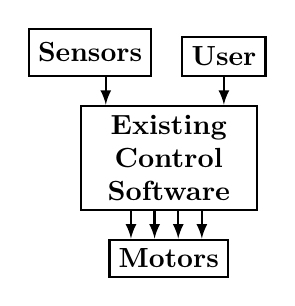
\begin{tikzpicture}
    \tikzstyle{every node}=[draw=black,thick,font=\bfseries,node distance=0.35cm]
    \tikzstyle{every path}=[draw=black,thick]
    \tikzstyle{wnode}=[minimum width=1cm]

    \node[wnode,text width=2cm,align=center] (existing)  {Existing Control Software} ;

    \node[draw=black,above=of existing,minimum height=0.5cm,xshift=0.7cm] (user) {User} ;
    \node[draw=black,above=of existing,minimum height=0.6cm,xshift=-1cm] (sensor) {Sensors} ;

    \node[wnode,below=of existing] (motor)  {Motors} ;

    \newcommand{\quadline}[2]{%
    \foreach \i in {-2,...,1}{%
      \draw[-latex] ([xshift=0.12cm + \i * 0.3 cm]#1.south) -- ([xshift=0.12cm + \i * 0.3 cm]#2.north) ;}}

    \quadline{existing}{motor}
    \draw[-latex] let \p1 = (user.south),
                      \p2 = (existing.north) in
                  (user.south) -- (\x1,\y2) ;
    \draw[-latex] let \p1 = (sensor.south),
                      \p2 = (existing.north) in
                  ([xshift=0.2cm]sensor.south) -- (\x1+0.2cm,\y2) ;



  \end{tikzpicture}
  \caption{}
  \label{fig:memo15-arch-without}
\end{subfigure}
~
\begin{subfigure}[t]{.49\linewidth}
  \centering
  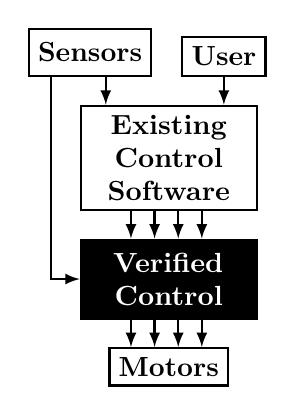
\begin{tikzpicture}
    \tikzstyle{every node}=[draw=black,thick,font=\bfseries,node distance=0.35cm]
    \tikzstyle{every path}=[draw=black,thick]
    \tikzstyle{wnode}=[minimum width=1cm]

    \node[fill=black,text=white,text width=2cm,align=center,minimum height=1cm] (mon) at (0,0) {Verified Control} ;
    \node[wnode,above=of mon,text width=2cm,align=center] (existing)  {Existing Control Software} ;

    \node[draw=black,above=of existing,minimum height=0.5cm,xshift=0.7cm] (user) {User} ;
    \node[draw=black,above=of existing,minimum height=0.6cm,xshift=-1cm] (sensor) {Sensors} ;

    \node[wnode,below=of mon] (motor)  {Motors} ;

    \newcommand{\quadline}[2]{%
    \foreach \i in {-2,...,1}{%
      \draw[-latex] ([xshift=0.12cm + \i * 0.3 cm]#1.south) -- ([xshift=0.12cm + \i * 0.3 cm]#2.north) ;}}

    \quadline{mon}{motor}
    \quadline{existing}{mon}
    \draw[-latex] let \p1 = (user.south),
                      \p2 = (existing.north) in
                  (user.south) -- (\x1,\y2) ;
    \draw[-latex] let \p1 = (sensor.south),
                      \p2 = (existing.north) in
                  ([xshift=0.2cm]sensor.south) -- (\x1+0.2cm,\y2) ;
    \draw[-latex] ([xshift=-0.5cm]sensor.south) |- (mon.west) ;


  \end{tikzpicture}
  \caption{}
  \label{fig:memo15-arch-with}
\end{subfigure}

\caption{A simplified depiction of UAV architecture~\ref{fig:memo15-arch-without} without and~\ref{fig:memo15-arch-with} with one of our controllers.}
\label{fig:arch-shim}
\end{figure}

\section{Model and Verification}
\label{sec:memo15-model}
We now focus on our controller that ensures the velocity of a simple
one-dimensional model of a quadcopter never exceeds a constant upper bound
\ub{}. We start by modeling the system using our abstraction \SysA{}
(Definition~\ref{def:sys-abstraction}), present our sampled-data induction
rule, and demonstrate how to use this rule to verify the safety invariant
of the velocity bounding controller. In
Section~\ref{sec:memo15-composition}, we will present our composition rule
and show how to use it to verify safety in the presence of sensor error and
delay.

\subsection{Model}
Our velocity controller makes use of the following variables (by
convention, lower case variables are continuous and upper case variables
are discrete): $\V$ is the actual velocity of the system, whose behavior
will be specified by differential equations encoding the physics of the
real world; $\Vmax$ is an upper bound on $\V$ (e.g. produced by a sensor)
and is an input to our controller; $\Tproposed$ is the thrust requested by the
higher level controller, which is also an input to our controller; $\T$ is the
thrust produced by our controller, which gets sent to the motors. Our controller is
defined as follows:
\[
\VelShim \defined \Sys{D}{\W}{\Delta}
\]
where
\[
\begin{array}{rcl}
\W & \defined & \dt{\V}\leq\T - g \\
D & \defined & ((\Tproposed-g)\cdot\Delta + \Vmax \leq \ub \wedge \T\tlaprime {=} \Tproposed) \vee \T\tlaprime {=} g
\end{array}
\]
$\W$ states the differential inequality capturing how velocity is related
to thrust ($\T$) and gravity ($g$).  This relationship is an inequality
rather than an equality because we are modeling a quadcopter, whose
vertical thrust is only upper-bounded by the thrust produced by the motors.
We discuss this further in Section~\ref{sec:experiences}.  The action
formula $D$ captures the control logic of our controller.  The disjunction
encodes, essentially, the following conditional statement:
$\texttt{if}\,\Tproposed \cdot \Delta + \Vmax \leq
\ub\,\texttt{then}\,\T\tlaprime = \Tproposed\,\texttt{else}\,\T\tlaprime =
g$; though it also allows executing the safe action ($\T\tlaprime = g$)
when the check succeeds.

Since \SysA{} unfolds directly to an LTL formula, we can express the
correctness of our controller directly in LTL as follows, where $\entails$
(Definition~\ref{def:ltl-entails}) represents entailment in LTL, expressing
that the formula to the right of the $\entails$ holds on all traces
satisfying the formula to the left of the $\entails$:
\begin{align}
\label{thm:shim-safe}
\Always{\V \leq \Vmax} \vdash \Init \wedge \VelShim \rightarrow \Always{\V \leq \ub} \\
\Init \defined \max(0,\T - g )\cdot\Delta + \V \leq \ub \nonumber
\end{align}
This formula states that if $\Vmax$ is always an upper bound on the actual
velocity ($\Always{\V \leq \Vmax}$), then the velocity controller ensures
that the velocity of the system is always less than or equal to \ub{}.
This requires a predicate on the initial state, given by \Init, which
states that the velocity is at most \ub{} and furthermore is small enough
that it will still be at most \ub{} when the controller first runs (which
will be at most $\Delta$ time units away).  For now, we do not specify how
the value of $\Vmax$ is produced; that is, $\Vmax$ does not appear in any
action formulas (transitions).  Instead, we simply assume that such a value
is provided to the controller.  In Section~\ref{sec:compose}, we will show
how to specify systems that produce a $\Vmax$ satisfying this assumption
and we will show how to compose them with the velocity controller.

\subsection{Proof}
We now show how we prove the above LTL formula in Coq.  To do so, we need
an inductive invariant that is preserved both by the continuous transitions
(those of the world) and the discrete program.  Although we have
implemented several mechanisms for simplifying reasoning about \SysA{}, we
currently do not infer invariants automatically. In the case of the
velocity controller, the inductive invariant is relatively simple: the
velocity cannot violate the upper bound before the next execution of the
controller:
\[
\max(0,\T - g)*\Time + \V \leq \ub
\]
Here, the variable \Time{}, introduced in
Definition~\ref{def:sys-abstraction} tracks the maximum amount of time
until the next execution of the controller.

In order to prove that this formula is an inductive invariant, we use the
the \textsc{SysInd} proof rule (Theorem~\ref{thm:sys-ind}), which is a
special case of discrete induction tailored to systems that are described
by our \SysA{} construct.  Proof rules such as this one allow us to
abstract the implementation of \SysA{} and make for overall cleaner proofs.
Informally, \textsc{SysInd} states that a formula $P$ is an (inductive)
invariant of a system if $P$ holds on all possible initial states of the
system, and $P$ is preserved by the two possible transitions that the
system can make.  We use $P\tlaprime$ to denote the formula $P$ with all
unprimed variables $\tlavar{x}$ replaced with their primed counterpart
$\tlanextvar{x}$.

\begin{theorem}[\textsc{SysInd}]
For state formulas $P,Q,I$, action formula $D$, constant $\Delta \in \R$,
and evolution predicate $\W$, if the following conditions hold:

\begin{enumerate}[label=\roman*), ref=\roman*]
\item
\label{thm:sys-ind-init}
$Q~\entails 0 \leq \Time \leq \Delta~\wedge~I \rightarrow P$
\item
\label{thm:sys-ind-discr}
$Q~\entails 0 \leq \Time{} \leq \Delta~\wedge~P~\wedge~D~\wedge~\tlanextvar{\Time{}} = \Time{} \rightarrow \Next{P}$
\item
\label{thm:sys-ind-cont}
$Q~\entails \Time \leq \Delta~\wedge~0 \leq \tlanextvar{\Time}~\wedge~P~\wedge~\Continuous{(\W)} \rightarrow \Next{P}$
\end{enumerate}
then
\[
\Always{Q}~\entails I~\wedge~\Sys{D}{\W}{\Delta} \rightarrow \Always{P}
\]
\label{thm:sys-ind}
\end{theorem}

To illustrate how the proof works, we walk through the proof obligations
obtained by applying \textsc{SysInd} to our velocity controller.  First, we
must prove that $P$ holds on all initial states of the system:
\[
\begin{array}{lc}
\V \leq \Vmax & \vdash \left[
\begin{array}{ll}
& 0 \leq \Time \leq \Delta \\
\wedge & \max(0,\T - g )\cdot\Delta + \V \leq \ub \\
\rightarrow & \max(0,\T - g)\cdot\Time + \V \leq \ub
\end{array}
\right]
\end{array}
\]
Proving this requires first order reasoning over real arithmetic in Coq.
We can solve simple obligations such as this one, using existing Coq real
arithmetic decision procedures~\cite{besson2007micromega} that produce
foundational Coq proofs completely automatically.  While these procedures
are not complete, they are still able to discharge many obligations that
arise in practice.  When they are unable to completely prove a goal, we are
forced to manually construct a machine-checked proof of the remaining
obligations. This requires manual application of real arithmetic lemmas
such as transitivity of comparison operators. This can become quite tedious
as the system becomes more complex.  The compositional reasoning
techniques, which we describe in Section~\ref{sec:memo15-composition}, help
to reduce this burden by producing smaller arithmetic goals that only deal
with a part of the system. We discuss this benefit in more detail in
Section~\ref{sec:height-shim}.

Next, we prove that the inductive invariant is preserved by discrete steps
of the system.  There are actually two cases to prove: when the proposed
thrust passes the controller's safety check and when the controller issues
a thrust equal to gravity.  In the first case, we are left to prove the
following proof obligation (the reasoning in the second case is simpler):
\[
\begin{array}{lc}
\V \leq \Vmax & \vdash \left[
\begin{array}{ll}
& 0 \leq \Time \leq \Delta \\
\wedge & \max(0,\T - g)*\Time + \V \leq \ub \\
\wedge & (\Tproposed-g)*\Delta + \Vmax \leq \ub \\
\wedge & \T\tlaprime = \Tproposed  \\
\wedge & \V\tlaprime = \V \\
\wedge & \Time\tlaprime = \Time \\
\rightarrow & \max(0,\T\tlaprime - g)*\Time\tlaprime + \V\tlaprime \leq \ub
\end{array}
\right]
\end{array}
\]
Proving this obligation requires first order reasoning over real
arithmetic, but fits into the automation described above.

Finally, we prove that the inductive invariant is preserved by continuous
transitions.  This proof obligation is slightly more difficult:
\[
\begin{array}{lc}
\V \leq \Vmax & \vdash \left[
\begin{array}{ll}
& \Time \leq \Delta \wedge 0 \leq \Time\tlaprime \\
\wedge & \max(0,\T - g)\cdot\Time + \V \leq \ub \\
\wedge & \Continuous{(\W)} \\
\rightarrow & \max(0,\T\tlaprime - g)\cdot\Time\tlaprime + \V\tlaprime \leq \ub
\end{array}
\right]
\end{array}
\]
Continuous evolution of the physical world is expressed by the formula
$\Continuous{(\W)}$ (Definition~\ref{def:continuous}). We prove this
obligation using our adaptation of Platzer's differential induction proof
rule~\cite{platzer2010logical}, which justifies a technique for proving
invariants of a system of differential equations without computing an
explicit solution.  Roughly speaking, differential induction captures the
fact that $e_1 \leq e_2$ is preserved by a continuous transition
(e.g. $\Continuous{(\W)}$) if the derivative of $e_1$ is less than or equal
to the derivative of $e_2$, under the constraints given by $\W$.  Applying
differential induction leaves us to prove a first order formula over real
arithmetic that the automation can solve with a minimal amount of
assistance.

Proving these four goals completes the proof
of~\eqref{thm:shim-safe}. Since the inductive invariant was simple and the
arithmetic reasoning was within the scope of Coq's built-in automation,
this proof was relatively easy. However, the proof demonstrates the general
mechanics of proving an invariant of a periodic sampled-data system and
illustrates how \textsc{SysInd} abstracts some of the tedious reasoning
common to all such systems.

\section{Composition}
\label{sec:memo15-composition}
While the velocity controller does guarantee the safety property, it
requires an assumption about an input, namely that $\V \leq \Vmax$.  We
could modify the specification of the velocity controller so that it
specifies the transition behavior of $\Vmax$ in a way that guarantees that
$\V \leq \Vmax$, thus removing the assumption.  That is, we could modify
the controller specification to show how $\Vmax$ is produced by adding
$\Vmax$ to action formulas of the specification.  However, this would
require reproving the safety theorem of the velocity controller
(formula~\eqref{thm:shim-safe}).  By leaving the sensor under-specified in
the velocity controller, we are able to compose the velocity controller
with \emph{any} system that guarantees $\Always{\V \leq \Vmax}$, without
needing to reprove the safety theorem of the velocity controller.  In this
section, we show how to do this for several examples, using a general
composition rule for our \SysA{} abstraction.

\subsection{Sensor Error}
Real sensors always have some notion of error.  For example, the readings
from a barometer may be affected by pressure differences due to local
weather or GPS may only give accurate information to within several feet.
In addition, sensors, detect physical, continuous values and compute
discrete approximations of these values, for example using fixed- or
floating point.  These finite representations can not hope to be exactly
the true values of the variables they represent.  While the first type of
error can be modeled probabilistically, we assume that a sensor can be
assigned a deterministic conservative upper bound on the error. Thus, it is
easy to model both kinds of error in our framework since we only need to
specify predicates on the sensed values.

We start with a simple specification of a sensor that can read the value of
$\V$ to within some error $\epsilon$.  To do so, we first define
$\Sensor{S}{\W}{\Delta}$, which takes an LTL state formula $S$ and a
positive number $\Delta$, and produces an LTL formula:
\[
\Sensor{S}{\W}{\Delta} \defined \Sys{(\Unchanged{\vars{\W \wedge S}})}{(\W \wedge S)}{\Delta}
\]
This formula expresses the system in which $S$ holds throughout every
continuous transition, and all variables in the continuous transition are
unchanged by the discrete transition. The action formula expressing that
all variables in the continuous transition are unchanged is given by
$\Unchanged{\vars{\W~\wedge~S}}$. In the actual Coq implementation, the set
of variables must be supplied manually.

Intuitively, $S$ is intended to express the relationship between the
physical variable that the sensor is tracking and the actual value it
reads.  For a sensor of some physical variable $\X$, this relationship is
$\X - \epsilon \leq \Xsense \leq \X + \epsilon$, where $\Xsense$ is the
sensed value.  However, for our purposes, we actually need an upper bound
on $\X$, which we accomplish by offsetting $\Xsense$ by $\epsilon$:
\[
\Sense{\X}{\Xmax} \defined
\X - \epsilon \leq \Xsense \leq \X + \epsilon~\wedge~\Xmax = \Xsense + \epsilon
\]

In order to satisfy the assumption of the velocity controller, we
instantiate $\SenseA{}$ with $\V$ and $\Vmax$ and need to prove that for
any $\W$, $\Delta$, and $\epsilon \geq 0$,
\begin{equation}
\vdash \Sense{\V}{\Vmax}~\wedge~\Sensor{\Sense{\V}{\Vmax}}{\W}{\Delta} \rightarrow \Always{\V \leq \Vmax}
\label{thm:sense-safe}
\end{equation}
This theorem follows from \textsc{SysInd} and simple reasoning about linear
real arithmetic.

\subsection{Composition}
We are now in a position to compose the sensor module with our velocity
controller.  First, let \SysA{} composition (\SysConjoin{}) be defined by
conjoining corresponding formulas:
\begin{restatable}{definition}{sysconjoin}{Conjunctive composition}
\[
\SysConjoinP{\Sys{D_1}{\W_1}{\Delta}}{\Sys{D_2}{\W_2}{\Delta}} \defined \Sys{\left(D_1 \wedge D_2\right)}{\left(\W_1 \wedge W_2\right)}{\Delta}
\]
\end{restatable}
Note that since all LTL formulas operate on the same state variables,
conjunction is a very general notion of composition.

Using the definition of \SysConjoin{}, we can state the theorem that the
composition of our sensor with our velocity controller satisfies the safety
property $\Always{\V \leq \ub}$ without any assumptions on $\Vmax$:
\[
\vdash \SysConjoinP{\Sensor{\Sense{\V}{\Vmax}}{\W}{\Delta}}{\VelShim} \rightarrow \Always{\V \leq \ub}
\]
This theorem follows immediately from \textsc{SysCompose}
(Theorem~\ref{thm:sys-compose}).  \textsc{SysCompose} states that if the
first system guarantees an invariant, then the second system can assume
that invariant when it proves its safety condition.  The combined system
does not need the assumption; it has been satisfied by the first system,
and has both properties.  Similar to \textsc{SysInd}, \textsc{SysCompose}
abstracts all of the reasoning for manipulating the internals of the
\SysA{} abstraction.  Crucially, when we apply \textsc{SysCompose}, we do
not need to reprove any theorems about the two systems.  Instead we can
simply use the soundness proofs of the components to satisfy the premises
of \textsc{SysCompose}.

\begin{theorem}[\textsc{SysCompose}]
For state formulas $P,Q,I_a,I_b$, action formulas $D_a,D_b$, constant $\Delta \in \R$,
and evolution predicate $\W$, if the following conditions hold:

\begin{enumerate}[label=\roman*), ref=\roman*]
\item
\label{thm:sys-compose-a}
$\entails I_a~\wedge~\Sys{D_a}{\W}{\Delta} \rightarrow \Always{P}$
\item
\label{thm:sys-compose-b}
$\Always{P} \entails I_b~\wedge~\Sys{D_b}{\W}{\Delta} \rightarrow \Always{Q}$
\end{enumerate}
then
\[
\entails I_a~\wedge~I_b~\wedge~\SysConjoinP{\Sys{D_a}{\W}{\Delta}}{\Sys{D_b}{\W}{\Delta}} {\rightarrow} \Always{(P \wedge Q)}
\]
\label{thm:sys-compose}
\end{theorem}

\subsection{Delay Compensation}
\label{sec:delay-comp}
When we compose the sensor specification with the velocity controller, we
implicitly assume that the velocity controller can instantaneously read and
compute with the value produced by the sensor module, $\Vmax$.  In reality,
due to communication or computation time, this may not be the case.  It may
be the case that there is some delay between when the sensor module
produces a value and when it can actually be used in the controller's
safety check.  For example, suppose that the sensor module actually outputs
some value, represented by the variable $\Vmaxpre$ that cannot
instantaneously be used in a safety check.  The following system
compensates for this delay
\[
\DelayComp \defined \Sys{D}{\W}{\Delta}
\]
where $\W \defined \dt{\V}\leq\T - g$ as before and
\[
D  \defined \Vmax\tlaprime = \Vmaxpre + \Delta \cdot \mathsf{max}(0, \T\tlaprime - g)
\]
In this system, $D$ uses the current value of $\Vmaxpre$ to compute an
upper bound on $\V$ for the next $\Delta$ time.
%% , and sets $\Vmax$ equal to it. %% , which can then be used during the
%% next discrete transition.  Here, $\Vmax\tlaprime$ is set to a value that
%% will be an upper bound on $\V$ for the next $\Delta$ time.

The correctness property for this system is
\begin{align}
\Always{\V \leq \Vmaxpre} \entails I~\wedge~\DelayComp \rightarrow \Always{\V \leq \Vmax} \\
I \defined \Vmax = \V + \Delta \cdot \mathsf{max}(0, \T - g) \nonumber
\label{thm:delay-safe}
\end{align}

Notice that this property relies on the assumption $\Always{\V \leq
  \Vmaxpre}$.  However, we can use the sensor module above to satisfy this
assumption and use \textsc{SysCompose} to verify the combined system
without any assumptions, again without reproving the properties of the
individual systems:
\[
\entails \SysConjoinP{\Sensor{\Sense{\V}{\Vmaxpre}}{\W}{\Delta}}{\DelayComp} \rightarrow \Always{\V \leq \Vmax}
\]
Now we have a new system that guarantees the assumption of the velocity
controller, so we can compose them and easily prove the theorem:
\[
\entails \SysConjoinP{\SysConjoinP{\Sensor{\Sense{\V}{\Vmaxpre}}{\W}{\Delta}}{\DelayComp}}{\VelShim} \rightarrow \Always{\V \leq \ub}
\]
This approach can be continued for any other sensors or full-blown
controllers that can be specified and verified within the \SysA{}
abstraction.

\subsection{Height controller}
\label{sec:height-shim}

In addition to controlling velocity through a first-derivative, we have
used our deductive approach to control position through a second
derivative.  In this section we describe our implementation of a controller
to enforce an upper bound on height by controlling acceleration.  Note that
if we were able to directly set the velocity then we could reuse the
velocity controller (and its proof) simply by renaming the variables.
Since directly setting velocity is unrealistic, we built a new controller
that bounds position by setting its second derivative.
\[
\HeightShim \defined \Sys{D}{\W}{\Delta}
\]
where
\[
\begin{array}{rl}
\W &\defined \dt{\Y} = \V,~\dt{\V}\leq\T - g \\
D &\defined \quad \tdist{\Vmax}{a_c}{\Delta} {+} \sdist{\Vmax {+} a_c\Delta}{+}  \Ymax \leq \ubY~\wedge~\T\tlaprime {=} \Tproposed \\
   & ~~~~\vee~~\T\tlaprime {=} \amin \\
\tdist{\V}{\T}{\Delta} &\defined \V\cdot\Delta+\frac{\T\Delta^2}{2} \\
\sdist{\V} &\defined -\frac{\V^2}{2\cdot(\amin - g)} \\
a_{c}  &\defined \max(0,\Tproposed - g ) \qquad \amin  < g
\end{array}
\]
The approach is similar to the approach of the velocity controller.  Each
time this controller runs, it checks whether it will be able to stop in
time if it issues the maximum breaking acceleration ($\amin$) the next time
the controller runs.  The function $\mathsf{td}$ computes a conservative
upper-bound on the height at the end of $\Delta$ time and $\mathsf{sd}$
computes the stopping distance assuming $\amin$ breaking acceleration.  We
have formally proven that the height controller guarantees that $\Y$ never
exceeds $\ubY$, under the assumption that $\Ymax$ and $\Vmax$ are bounds on
their respective physical variables.  Formally,
\[
\Always{(\Y \leq \Ymax \wedge \V \leq \Vmax)} \entails \HeightShim \rightarrow \Always{\Y \leq \ubY}
\]
As with the velocity controller, we can compose the height controller with
modules guaranteeing the assumptions that the height controller makes on
$\Ymax$ and $\Vmax$.  Using \textsc{SysCompose}, we can easily prove that
the composed system guarantees $\Always{\Y \leq \ubY}$ from the individual
proofs, without reasoning simultaneously about the entire composed system
and without reproving anything about the individual parts.

Verifying the height controller differs from the velocity controller in two
ways.  First, the differential equations describing the physical evolution
of the system, the controller logic, and therefore the inductive invariant
are all more complex.  This in turn means that the real arithmetic proof
obligations are substantially more intricate.  In practice, this means that
the existing foundational, nonlinear real arithmetic decision procedure is
not able to solve all of the goals, even though the unverified SMT solver
Z3~\cite{demoura2008z3} solves all goals quickly.  Second, the verification
used history variables (omitted from the specification in this paper for
simplicity) to record the value of each physical variable in the last
discrete transition.  We use these values to describe the safety buffer
that the system consumes during the continuous transition.  These variables
do not change the behavior of the controller in any way; they are used only
for reasoning.

\paragraph*{Benefits of Composition}
When verifying our two controllers, the vast majority of the verification
effort was devoted to foundationally reasoning about real arithmetic proof
obligations.  Our composition technique takes a step towards reducing that
burden.  As a point of comparison with the non-compositional approach, our
first implementation of the height controller was monolithic, including all
of the code for reasoning about delay compensation (but not sensor error).
The result was more complex real arithmetic goals containing larger
expressions and more variables.  When we verified the height controller
compositionally, the arithmetic proof obligations were simpler and, as a
result, required less manual proof effort to simplify the goals into a form
that the foundational decision procedures could handle.  Moreover,
verifying the height controller with the noisy sensor was simply a matter
of combining the independent proofs using \textsc{SysCompose}.  This is a
promising result considering that the number of variables influences the
complexity of the inductive invariant which is directly related to
complexity of automatic verification and difficulty of manual arithmetic
proofs when automation fails.

\paragraph*{Finding Inductive Invariants}
In general, one of the challenges of formal verification lies in building a
suitable inductive invariant, and hybrid systems are no exception.
However, we have found that developing the inductive invariant is actually
a part of the process of developing the controller.  For example, when
building the velocity controller, we first built the inductive invariant
stating that the thrust is safe until the next time the controller runs.
We then built a controller to compute a thrust that will be safe until the
next time it runs; this followed naturally from the inductive invariant.
This means that we have not found the task of finding an inductive
invariant to be an \emph{additional} burden on top of the necessary task of
building the controller itself. Instead, we found these two tasks to be
naturally related, regardless of whether or not one performs foundational
verification.

\section{From Model to Reality}
\label{sec:experiences}
In addition to modeling and verifying our systems, we also implemented both
the velocity and height controllers to run on a 3D Robotics Iris+.  Running
the system whose model we verify is important because it allows us to
experimentally evaluate the gap between the model and the actual system
that we run.  We can divide this gap into two pieces: the gap due to our
model of the physical world (Section~\ref{sec:world-model}), and the gap
due to our model of the discrete controller
(Section~\ref{sec:discrete-model}).  We conclude by discussing some of the
insights that we gained from running our code on an actual quadcopter
(Section~\ref{sec:results}).

\subsection{A Small Model in a Big World}
\label{sec:world-model}

The primary gap between the physical world and our model lies in the fact
that our model captures only the vertical dimension.  In particular, it
does not model the orientation of the quadcopter and therefore does not
capture the direction of thrust.  However, a model that includes attitude
is a refinement of the world model that our specifications use.  This means
that all traces allowed by a model including attitude are also allowed by
the world model used in our specifications.  As we explained in
Section~\ref{sec:sys}, this is because our specifications model the world
using differential \emph{inequalities} stating that the vertical thrust is
upper-bounded by the thrust produced by the motors.  This relaxation of the
specification means that we must prove properties of a more liberal system,
but it allows us to use our results in the more constrained, richer model
which includes attitude.

The other discrepancies between our model and the real world are common
simplifying assumptions of models for verification purposes.  For example,
modeling external factors such as wind, air resistance, etc. would be
possible by adding extra terms into the differential world description.
Finally, our model also relies on the common assumption of instantaneous
change of discrete variables such as thrust.  In principle, output values
such as thrust actually change over a very small amount of time.  While
this may seem like a reasonable assumption, it nonetheless constitutes a
formal discrepancy.

\subsection{From Relations to Bits}
\label{sec:discrete-model}

Our description of the autpilot architecture in Section~\ref{sec:example}
describes the verified controller as the last piece of code that runs
before signals are sent to the motors.  This is not strictly necessary.
There are advantages and disadvantages to running the verified controller
at different points.


\begin{figure}[t]
\centering

\begin{subfigure}[t]{.3\linewidth}
  \centering
  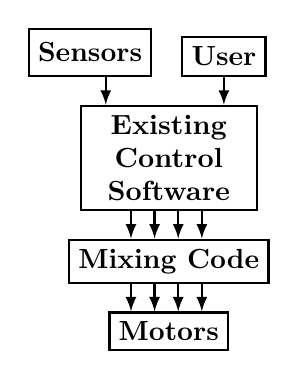
\begin{tikzpicture}
    \tikzstyle{every node}=[draw=black,thick,font=\bfseries,node distance=0.35cm]
    \tikzstyle{every path}=[draw=black,thick]
    \tikzstyle{wnode}=[minimum width=1cm]

    \node[wnode,text width=2cm,align=center] (existing)  {Existing Control Software} ;

    \node[draw=black,above=of existing,minimum height=0.5cm,xshift=0.7cm] (user) {User} ;
    \node[draw=black,above=of existing,minimum height=0.6cm,xshift=-1cm] (sensor) {Sensors} ;

    \node[wnode,below=of existing] (mixing)  {Mixing Code} ;
    \node[wnode,below=of mixing] (motor)  {Motors} ;

    \newcommand{\quadline}[2]{%
    \foreach \i in {-2,...,1}{%
      \draw[-latex] ([xshift=0.12cm + \i * 0.3 cm]#1.south) -- ([xshift=0.12cm + \i * 0.3 cm]#2.north) ;}}

    \quadline{existing}{mixing}
    \quadline{mixing}{motor}
    \draw[-latex] let \p1 = (user.south),
                      \p2 = (existing.north) in
                  (user.south) -- (\x1,\y2) ;
    \draw[-latex] let \p1 = (sensor.south),
                      \p2 = (existing.north) in
                  ([xshift=0.2cm]sensor.south) -- (\x1+0.2cm,\y2) ;



  \end{tikzpicture}
  \caption{}
  \label{fig:memo15-arch-full-without}
\end{subfigure}
~
\begin{subfigure}[t]{.3\linewidth}
  \centering
  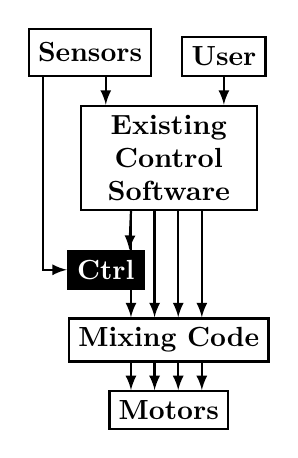
\begin{tikzpicture}
    \tikzstyle{every node}=[draw=black,thick,font=\bfseries,node distance=0.35cm]
    \tikzstyle{every path}=[draw=black,thick]
    \tikzstyle{wnode}=[minimum width=1cm]

    \node[wnode] (mixing)  {Mixing Code} ;
    \node[wnode,above=of mixing,text width=2cm,align=center,yshift=1cm] (existing)  {Existing Control Software} ;


    \node[draw=black,above=of existing,minimum height=0.5cm,xshift=0.7cm] (user) {User} ;
    \node[draw=black,above=of existing,minimum height=0.6cm,xshift=-1cm] (sensor) {Sensors} ;

    \node[wnode,below=of mixing] (motor)  {Motors} ;

    \newcommand{\quadline}[2]{%
    \foreach \i in {-2,...,1}{%
      \draw[-latex] ([xshift=0.12cm + \i * 0.3 cm]#1.south) -- ([xshift=0.12cm + \i * 0.3 cm]#2.north) ;}}

    \quadline{existing}{mixing}
    \quadline{mixing}{motor}
    \node[fill=black,above=of mixing,text=white,align=center,xshift=-.8cm] (mon) {Ctrl} ;
    \draw[-latex] let \p1 = (user.south),
                      \p2 = (existing.north) in
                  (user.south) -- (\x1,\y2) ;
    \draw[-latex] let \p1 = (sensor.south),
                      \p2 = (existing.north) in
                  ([xshift=0.2cm]sensor.south) -- (\x1+0.2cm,\y2) ;
    \draw[-latex] ([xshift=-0.6cm]sensor.south) |- (mon.west) ;
    \draw[-latex] let \p1 = (mon.north) in
                  ([xshift=-0.48cm]existing.south) -- (\x1+0.3cm,\y1) ;


  \end{tikzpicture}
  \caption{}
  \label{fig:memo15-arch-full-before}
\end{subfigure}
~
\begin{subfigure}[t]{.3\linewidth}
  \centering
  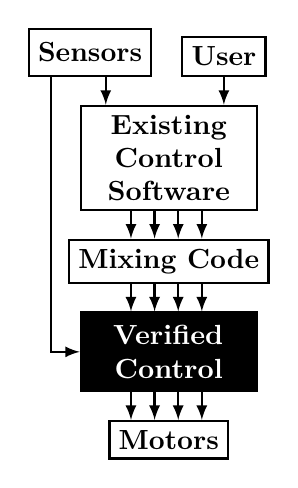
\begin{tikzpicture}
    \tikzstyle{every node}=[draw=black,thick,font=\bfseries,node distance=0.35cm]
    \tikzstyle{every path}=[draw=black,thick]
    \tikzstyle{wnode}=[minimum width=1cm]

    \node[fill=black,text=white,text width=2cm,align=center,minimum height=1cm] (mon) at (0,0) {Verified Control} ;
    \node[wnode,above=of mon] (mixing)  {Mixing Code} ;
    \node[wnode,above=of mixing,text width=2cm,align=center] (existing)  {Existing Control Software} ;

    \node[draw=black,above=of existing,minimum height=0.5cm,xshift=0.7cm] (user) {User} ;
    \node[draw=black,above=of existing,minimum height=0.6cm,xshift=-1cm] (sensor) {Sensors} ;

    \node[wnode,below=of mon] (motor)  {Motors} ;

    \newcommand{\quadline}[2]{%
    \foreach \i in {-2,...,1}{%
      \draw[-latex] ([xshift=0.12cm + \i * 0.3 cm]#1.south) -- ([xshift=0.12cm + \i * 0.3 cm]#2.north) ;}}

    \quadline{mon}{motor}
    \quadline{existing}{mixing}
    \quadline{mixing}{mon}
    \draw[-latex] let \p1 = (user.south),
                      \p2 = (existing.north) in
                  (user.south) -- (\x1,\y2) ;
    \draw[-latex] let \p1 = (sensor.south),
                      \p2 = (existing.north) in
                  ([xshift=0.2cm]sensor.south) -- (\x1+0.2cm,\y2) ;
    \draw[-latex] ([xshift=-0.5cm]sensor.south) |- (mon.west) ;


  \end{tikzpicture}
  \caption{}
  \label{fig:memo15-arch-full-after}
\end{subfigure}

\caption{A depiction of UAV architecture~\ref{fig:memo15-arch-full-without}
  without any modification, \ref{fig:memo15-arch-full-before} with our
  controller running before the motor mixing code, and
  \ref{fig:memo15-arch-full-before} with our controller running after the
  motor mixing code. Black boxes denote verified code.}
\label{fig:arch}
\end{figure}

Figure~\ref{fig:memo15-arch-full-without} depicts a version of the
\ardupilot{} architecture without any of our modifications.  The existing
control software takes input from the user and sensors and outputs a
desired throttle, roll torque, pitch torque, and yaw torque to the ``motor
mixer'' module.  This module then computes the signals to send to each of
the four motors to best approximate the desired behavior.  The
approximation is necessary because it is not always possible to achieve all
four desired values simultaneously since the quadcopter relies on
differences between motor speeds to induce non-zero torques.

One place to execute our controller is before the motor mixing module
(Figure~\ref{fig:memo15-arch-full-before}).  At this point, our controller
executes directly on the desired throttle of the higher-level controller.
To meet the interface of our specifications of both the height and velocity
controllers, we must convert this input into a desired vertical thrust
($\Tproposed$).  We must also convert the thrust output by the controllers ($\T$)
into a desired throttle that serves as the input to the mixer module.  We
accomplish both tasks by multiplying the throttle by a constant which we
determined empirically.  We discuss the consequence of this choice in
Section~\ref{sec:results}. As we have already discussed, this will actually
provide an upper bound on vertical acceleration, an acceptable input to our
controllers.  Placing the controller here allows the motor mixer to optimize the engine
outputs to achieve the other parameters (attitude torques) as best it can.
However, it also requires us to trust that the motor mixer module never
exceeds the desired throttle, a property that we believe to hold but have
not formally verified.

Running after the motor mixer (Figure~\ref{fig:memo15-arch-full-after})
allows us to remove the mixer from the trusted computing base.  To meet the
interface at this level, we must translate between the motor signals and
the induced thrust.  We again accomplish this using an empirically
determined constant that we use to scale each of the motor signals.  If the
controller rejects the proposed thrust, then it must compute new signals
for the motors to induce a safe thrust.  There are many ways to achieve a
particular total thrust by adjusting four motor signals.  In order to
minimize the affect of the controller on attitude dynamics, we linearly
scale back each of the motor values to achieve the thrust output by the
controller.

Regardless of where we insert the controller, the trusted computing base
still includes the sensor fusion code that runs on the quadcopter. This
code takes input from sensors and computes an estimation of the state
(e.g. position, velocity, attitude, etc.) of the vehicle. We use this code
to provide bounds ($\Vmax$ and $\Ymax$) on physical variables, in essence
treating the sensor fusion code as an unverified sensor module.  This code
is substantially larger and more complex than the motor mixing code and we
are interested in applying our techniques to reason about it in the future.
We are also trusting our (currently manual) translation of the discrete
controller model from LTL to C code.  This translation includes picking an
appropriate value for $\Delta$, the maximum time between discrete
transitions.  However, any upper bound suffices since our proofs hold for
all $\Delta$.  Finally, we ignore the formal gap between real arithmetic
used in our models and floating-point arithmetic used in the running code.
Future work can investigate closing this formal gap using Coq's libary for
reasoning about floating point computation~\cite{flocq11}.

\subsection{Empirical Results}
\label{sec:results}
Evaluating empirical results of this nature is important when exploring
models.  For example, when we first described our controller logic to an expert
pilot he was concerned that disengaging the motors so harshly might have a
destabilizing effect on the quadcopter.  It was only experimentally that we
learned that this was not the case.

Experimentally, both the velocity and the height controller enforce their
respective safety properties.  The height and velocity controllers allowed
the quadcoptor to go right up to the provided height or velocity bounds.
In some rare cases, the quadcopter went above the bounds, by a small
amount, for example about ten centimeters for a height bound of 30 meters.
We attribute these small violations to un-modeled forces such as wind,
sensor inaccuracy, and inaccuracy in the measured relationship between
throttle/motor signals and thrust induced.  In fact, we found the measured
relationship between signals and thrust to have a significant impact on the
behavior of the quadcopter and was perhaps the greatest source of error
that we noticed.  We were careful to be conservative when measuring these
constants; since our controllers both provide upper bounds, we can safely
err on the side of constants that provide upper bounds on acceleration.
Future work can investigate running our controllers on top of closed-loop
acceleration controllers to avoid the need for these empirical constants.

We flew the quadcopter in both loiter and stabilize modes, and also had the
quadcopter approach the height and velocity bounds from a variety of
velocities and orientations. In loiter mode, the pilot sends desired
velocity commands to the vehicle, while in stabilize mode, the pilot
commands desired attitudes. In all cases, the controllers enforced their
safety properties with rare, small violations, and allowed us to retain
control over the quadcopter.  We never ran both controllers simultaneously
because we have no verification results for this scenario.  Fundamentally,
to compose the controllers we are obliged to show that the controllers do
not conflict with one another, e.g. by requiring different remedial
actions. We investigate this further in Chapter~\ref{chap:emsoft16}.

Also, recall that our height controller is conservative in the way that it
estimates upward thrust: it assumes that the thrust requested by the
higher-level controller would be applied directly in the upward direction,
even if the attitude of the quadcoptor is not upward.  As a result, if the
attitude is not level, our height controller assumes that there is a larger
upward thrust than really occurs, and so it will engage earlier than it
needs to.  We noticed this effect experimentally: when approaching the
height through a non-level attitude, the quadcopter would stop ascending at
a lower height than the actual bound.  Furthermore, when the quadcopter is
at the height bound with the controller engaged and the upward throttle
stick engaged to the maximum, if we start rolling or pitching, the
quadcopter will not only move in the x-y direction, but it will also
descend slightly, since as the orientation changes, the height controller
becomes more conservative.

Finally, we also tried our velocity controller with a small negative
velocity as the bound. With the throttle stick engaged to the maximum, this
caused the quadcopter to land while allowing us to control other aspects of
the flight such as attitude and x-y positioning.

\section{Discussion}
\label{sec:discussion}

In this section we discuss the motivation for our design decisions.  We
begin by motivating the use of foundational proof assistants including some
anecdotal evidence for the benefits of foundational proofs. Next, we
describe the challenge of real arithmetic reasoning within a foundational
proof assistant. Finally, we discuss the design of our logic, particularly
the decision to use a global state.

\paragraph*{Benefits of foundational proof assistants}
\label{sec:proof-assistant}

Foundational proof assistants provide strong guarantees: they require all
proofs to be done in full formal detail, with an unparalleled attention to
every single detail.  This attention to detail can find subtle but critical
problems that otherwise might go unnoticed.  For example, we initially
axiomatized differential induction instead of proving it sound within our
framework.  We used this axiom to ``verify'' a version of the height
controller that was in fact not safe (note also that the height controller
itself is not trivial, and it is actually quite easy to get it wrong).
This left us in an unfortunate state of blissful ignorance: we had a subtle
bug in our controller, but we did not uncover it at first, \emph{even
  though we were applying formal methods}, because our statement of
differential induction was subtly incorrect, and we had not yet done the
foundational proof for differential induction.  It was only when we
attempted to foundationally prove, rather than axiomatize, differential
induction that we found our initial phrasing of the proof rule to be
unsound.  Fixing the statement led us to find several issues with earlier
versions of our formalism that appeared reasonable but were, in fact,
insufficiently constrained and therefore not correct.  These anecdotes
underscore the key benefit of foundational proofs: they provide a high
level of confidence, as has also been shown experimentally in previous
studies~\cite{yang2011understanding-compiler-bugs}.

In addition to the foundational guarantees, proof assistants provide very
expressive, general purpose logics, which can serve as the foundation of a
wide range of interesting theories.  We have leveraged the standard
library's real analysis theories to reason about real arithmetic and
calculus.  Future work can also make formal connections with actual
controller implementations, as the semantics of C~\cite{leroy2009compcert}
and floating point arithmetic~\cite{floqc11} are expressible. Furthermore,
as this dissertation emphasizes and future chapters reiterate, using Coq
allows us to use powerful, domain specific proof rules without sacrificing
soundness. In general, the full power of Coq's rich logic and all of the
theories built up in it are at our disposal.

The deductive reasoning style embodied in proof assistants provides useful
feedback when verification fails since the user is guiding the proof.  When
a proof does not work, the user is aware of all of the steps taken in the
development and often learns enough from the failed proof to be able to fix
the system.  This feedback is complementary to counter-examples provided by
tools such as Z3~\cite{demoura2008z3}, which do not provide foundational
proofs for nonlinear real arithmetic.  This process of building proofs also
makes the developer more aware of the minimal assumptions that a hybrid
system is making and the maximal guarantees that it can ensure.  In
practice, we have found that proofs lead us to find more general, and
therefore compositional, interfaces that are easier to satisfy.

Proof assistants also allow us to build automation without sacrificing
foundational proofs.  In this work, much of that automation surrounds our
embedding of temporal logic.  This automation is scripted in \ltac, which
means that the automation lies completely outside of our trusted computing
base.  This property has allowed us to rapidly iterate on the automation
without needing to worry about its soundness.

\paragraph*{Automation for real arithmetic}
The biggest drawback to the use of foundational proof assistants for
formalizing hybrid systems is the lack of good automation for reasoning
about real arithmetic.  For example, the only nonlinear real arithmetic
decision procedure currently implemented for Coq is
\texttt{psatz}~\cite{besson2007micromega} which can be extremely slow, even
for simple goals.  This is especially true when the goal is unprovable;
\texttt{psatz} can run for hours before overflowing the stack. Moreover,
\texttt{psatz} never returns a counter example, making it even more
challenging to debug false arithmetic conjectures.  This means that we
spent a lot of time trying to prove goals that are ultimately unprovable.
However, modern SMT solvers such as Z3, Yices, and CVC4 have good support
for reasoning about real arithmetic.  We eventually started passing real
arithmetic goals to Z3 to sanity check them before running them through
\texttt{psatz}.  The value of doing this throughout the development process
could easily be measured in hours (or days) of productivity gained.  Our
composition theorems are another step towards reducing the proof burden by
factoring the problem into more manageable pieces.  We believe that even
more abstraction is possible by codifying the ``tricks of the trade'' as
formal, general-purpose proof rules.

\paragraph*{Global state and unconstrainted transitions}
Unlike in a programming language where \texttt{x = y + 1} means that
\texttt{x} changes and the rest of the variables stays the same, in our
logic (like in TLA), $\tlanextvar{x} = \tlavar{y} + 1$ says nothing about
the behavior of variables other than $\tlavar{x}$ and $\tlavar{y}$. Thus,
other variables can transition arbitrarily.  This allows other components
to execute ``in parallel'' on their own state simply by joining the
programs using logical conjunction. In other words, parallel composition is
trivial to express. This, in turn, made it simple to express the definition
of $\SysConjoinP{}$ and reason about the composition of our height and
velocity controllers with sensor error and delay compensation. We will see
further benefits of this approach in Chapter~\ref{chap:emsoft16}.

The primary drawback to this approach is that care must be taken to avoid
these programs from interfering with one another in unexpected ways.  We
avoided this problem by enhancing our formalism with a mechanism for
renaming variables in LTL formulas. When one composes several components,
variable renaming must occur at the global level to avoid unintentional
conflicts. While this can be very tedious for programming languages, we
feel that for specifications like the ones in this dissertation, the
benefits outweight the drawbacks. However, more significantly,
Chapter~\ref{chap:emsoft16} will describe a specific pitfall that occurs
when composing components that \emph{intentionally} write to the same set
of variables.


\chapter{}
\label{chap:emsoft16}
Chapter~\ref{chap:memo15} introduced two atomic controllers that enforced
desired safety properties when run separately. That chapter also described
how to compose components, but informally followed the convention that
components being composed do not constrain overlapping sets of
variables. However, such a restriction is natural in sampled-data systems,
for example when composing two controllers outputing to the same sets of
actuators. This raises the question: when can two such controllers be run
in parallel in order to enforce the conjunction of their respective safety
properties? More generally, when can a sampled-data system be built up
modularly from smaller components while ensuring the properties guaranteed
by each of the components and avoiding inconsistencies in the composed
system? This chapter provides a series of proof rules to address that
question.

As alluded to above, one of the challenges is in ensuring that the
specification of the discrete controller is always enabled, i.e. it always
specifies at least one successor state.  While this might seem trivial,
consider the following scenario.  Suppose we have built a module that
prevents a quadcopter from exceeding some maximum altitude.  Furthermore,
suppose we have also built another module that prevents the quadcopter from
violating some \emph{minimum} altitude.  If we have separately verified
that these two modules enforce their respective properties, we would like
to compose them in parallel to guarantee both properties simultaneously.
That is, we would like the composed system to guarantee that the system
never goes too high or too low.  However, this is not always possible; a
module could enforce the upper bound on altitude by always accelerating
downwards.  Likewise, a module could enforce the lower bound on altitude by
always accelerating upwards.  Clearly, na\"ively composing the controllers
of these modules in parallel would result in a system that gets stuck --
there is never an acceleration that both controllers can agree on.

In this chapter, we present sound techniques for resolving this and other
potential pitfalls for reusing and composing modules for sampled-data
systems.  We observed that modularity is facilitated by separating
verification into two parts: \emph{preservation} and \emph{\progress{}}.
Preservation ensures that the model guarantees the safety property
inductively, while \progress{} ensures that the system model is always
enabled.  This separation facilitates the application of several simple,
general, and powerful operators, namely substitution, conjunction, and
disjunction.  More precisely, we state sufficient conditions for applying
these operators to individual modules to produce a new sampled-data system
with the desired properties (e.g. the conjunction of the safety properties
of conjoined modules).  Crucially, these sufficient conditions are in terms
of preservation and \progress{}.

To validate the expressiveness of our theorems, as in the rest of the
dissertation we apply them in the context of \emph{quadcopters}, by showing
how to compose several simple verified controllers together in different
ways to produce many different verified composed controllers.  To ensure
that our controllers are practical, we run them on an actual quadcopter.
In summary, the contributions of this chapter are:
\begin{itemize}
\setlength\itemsep{0.01em}
\item We implement in the Coq proof assistant a general approach for modular verification of sampled-data systems by separately exposing proofs of preservation and \progress{}. The development is available from the project webpage: \url{http://veridrone.ucsd.edu}.
\item We apply this approach to build and verify arbitrary 3D geofences for a quadcopter, including walls, boxes, and rectangular donuts, starting with two simple verified 1D controllers.
We show that our modular verification techniques keep the proof burden manageable.
\item We evaluate our geo-fences by running them on an actual quadcopter, and show that they work in practice.
\item We discuss the capabilities of three state-of-the-art fully-automated tools (SpaceEx, Flow*, and dReach) in verifying our geo-fence controllers.
\end{itemize}

\section{Overview}
We start with an informal description of the operators that our theory
covers: substitution, conjunction, and disjunction.  We then give an
overview of verifying controllers using these operators.  Finally, we
describe how we applied this to build a verified family of geo-fences for a
quadcopter.

\paragraph*{Operators}
\emph{Substitution} of expressions for variables represents a form of
reuse, allowing us to transform systems and their properties into a
different coordinate system.  For example, given a model of a system
defined in the x-y plane, the substitution $\{\tlavar{x} \mapsto \tlavar{r}
\cos \tlavar{\roll},\; \tlavar{y} \mapsto \tlavar{r} \sin \tlavar{\roll}\}$
transforms the model to polar coordinates, the substitution $\{\tlavar{x}
\mapsto \tlavar{y},\; \tlavar{y} \mapsto \tlavar{x}\}$ rotates the system,
and the substitution $\{\tlavar{x} \mapsto \tlavar{x} + 5\}$ translates the
system by 5 units in the $\tlavar{x}$ dimension.  However, not all
substitutions soundly transport both systems \emph{and} their properties;
our theory (Section~\ref{sec:subst}) gives formal conditions under which
substitutions are permitted.

\emph{Disjunction} of two systems represents nondeterministic choice
between the controllers of the system.  For example, if we have a
controller that prevents a quadcopter from flying too far to the west and
another controller that prevents a quadcopter from flying too far north,
then their disjunction enforces a north-west no-fly zone -- the quadcopter
must stay to the north \emph{or} to the west of the no-fly zone.  Unlike
conjunction, there is no risk of the composed system getting stuck.
Instead, the challenge with disjunction is in constraining the
nondeterministic choice between the controllers.  Our theorems and
definitions in Section~\ref{sec:disjunctive-composition} make this formal
by including the inductive invariants of each system within the composed
controller.

\emph{Conjunction} of two systems represents parallel composition of these
systems.  For example, if we have a system that enforces an upper bound on
velocity and a system that enforces a lower bound on velocity, then their
conjunction enforces both an upper and a lower bound on velocity.  We can
also conjoin systems that control or restrict different variables, such as
a system that enforces a bound on velocity and a system that enforces a
bound on position.  However, as discussed in the introduction, the
challenge of applying this operator is in ensuring that the conjoined
systems never get stuck, e.g. when the controller of one system requires
positive acceleration while the other requires negative acceleration.
Again, our theory (Section~\ref{sec:conjunctive-composition}) gives formal
conditions under which conjunctive composition is possible.

Note that disjunctive and conjunctive composition are related to
alternative and parallel composition.

\paragraph*{Controller Verification}
To illustrate how the operators work, we explain the construction and
modular verification of several general purpose controllers for enforcing
state constraints, depicted in Figure~\ref{fig:library}.  We begin with a
simple verified module: a controller that enforces an upper bound on
position in one spatial dimension by controlling acceleration (depicted by
(a) in Figure~\ref{fig:library}).  We use substitution to ``mirror'' this
module and its correctness property, thus obtaining a module (b) that
enforces a lower bound on position, again in one dimension.  We conjoin
these two modules to form a controller (c) enforcing upper and lower bounds
on position, still in one dimension.  We use substitution to rotate this
interval controller into a second, orthogonal dimension (d), then conjoin
(c) and (d) to form a controller (e) enforcing a 2 dimensional rectangle,
i.e. upper and lower bounds on position in two dimensions.  Finally, we use
substitution to build and verify four translated copies of (e) and
disjunction of these four copies to enforce a rectangular donut (f).  We
use disjunction to enforce that the system must, at all times, be in the
first copy of (e), the second, the third, \emph{or} the fourth.  Moreover,
since the rectangles are overlapping, the system can transition from one
rectangle to another.

\begin{figure}[t]
  \centering
  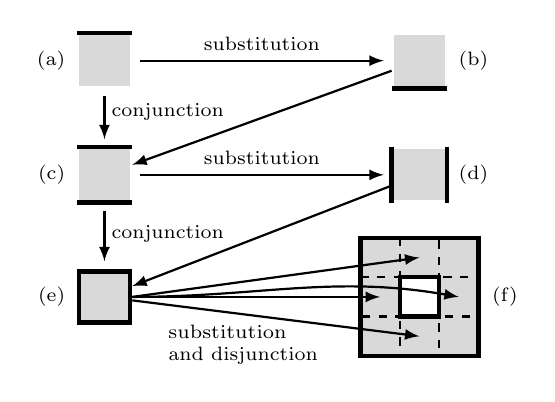
\begin{tikzpicture}
    \tikzstyle{every node}=[fill=black!15,node distance=0.5cm,font=\scriptsize]
    \tikzstyle{every path}=[draw=black,ultra thick]

   \node[draw=none,minimum height=0.65cm,minimum width=0.65cm,label=left:{(a)}] (y+) at (-2,2) {}
     (\tikzlastnode.north west)edge(\tikzlastnode.north east);

   \node[draw=none,minimum height=0.65cm,minimum width=0.65cm,label=right:{(b)}] (y-) at (2,2) {}
     (\tikzlastnode.south west)edge(\tikzlastnode.south east);

   \def\aoff{0.1};

   \draw[-latex,thick] ($(y+.east) + (\aoff,0)$) -- ($(y-.west) - (\aoff,0)$)
     node[draw=none,fill=none,font=\scriptsize,midway,above] {substitution};

   \def\coffx{0.35};
   \def\coffy{0.45};

   \node[draw=none,minimum height=0.65cm,minimum width=0.65cm,label=left:{(c)}] (y+-) at (-2,0.55) {}
     (\tikzlastnode.north west)edge(\tikzlastnode.north east)
     (\tikzlastnode.south west)edge(\tikzlastnode.south east)
     node[fill=none] at ($(y+-.north east) +(\coffx,\coffy)+(0.1,0)$) {conjunction};

   \draw[-latex,thick] ($(y+.south)-(0,\aoff)$) -- ($(y+-.north) + (0,\aoff)$);
   \draw[-latex,thick] (y-) -- (y+-);

   \node[draw=none,minimum height=0.65cm,minimum width=0.65cm,label=right:{(d)}] (x+-) at (2,0.55) {}
     (\tikzlastnode.north west)edge(\tikzlastnode.south west)
     (\tikzlastnode.north east)edge(\tikzlastnode.south east);

   \draw[-latex,thick] ($(y+-.east) + (\aoff,0)$) -- ($(x+-.west) - (\aoff,0)$)
     node[draw=none,fill=none,font=\scriptsize,midway,above] {substitution};

   \node[draw=black,ultra thick,minimum height=0.65cm,minimum width=0.65cm,label=left:{(e)}] (xy+-) at (-2,-1) {}
     node[fill=none] at ($(xy+-.north east) +(\coffx,\coffy)+(0.1,0)$) {conjunction};

   \draw[-latex,thick] ($(y+-.south) - (0,\aoff)$) -- ($(xy+-.north) + (0,\aoff)$);
   \draw[-latex,thick] (x+-) -- (xy+-);

   \node[draw=black,ultra thick,minimum height=1.5cm,minimum width=1.5cm,label=right:{(f)}] (donut_out) at (2,-1) {};
   \node[draw=black,ultra thick,fill=white,minimum height=0.5cm,minimum width=0.5cm] (donut_in) at (2,-1) {};
   \node[draw=black,thick,dashed,fill=none,minimum height=0.5cm,minimum width=1.5cm] (donut1) at (2,-0.5) {};
   \node[draw=black,thick,dashed,fill=none,minimum height=0.5cm,minimum width=1.5cm] (donut2) at (2,-1.5) {};
   \node[draw=black,thick,dashed,fill=none,minimum height=1.5cm,minimum width=0.5cm] (donut3) at (2.5,-1) {};
   \node[draw=black,thick,dashed,fill=none,minimum height=1.5cm,minimum width=0.5cm] (donut4) at (1.5,-1) {};

   \draw[-latex,thick] (xy+-.east) -- (donut1.center);
   \draw[-latex,thick] (xy+-) -- (donut2.center)
     node[draw=none,fill=none,font=\scriptsize,pos=0.4,below,text width=2cm] {substitution and disjunction};
   \draw[-latex,thick] (xy+-) edge[thick,out=0,in=170] (donut3.center);
   \draw[-latex,thick] (xy+-) -- (donut4.center);

  \end{tikzpicture}

     \caption{Overview of construction and verification of position bounding controllers.}
     \label{fig:library}
\end{figure}

\paragraph*{Quadcopter}
Although the above approach can enforce state constraints for a variety of
applications (e.g. trains, intelligent cruise control), we evaluate our
approach in the context of \emph{quadcopter} controllers that enforce
position and velocity bounds.  We performed this verification modularly
starting from two simple verified modules that we ported from prior work:
one enforcing an upper bound on velocity and another enforcing an upper
bound on position, both in one spatial dimension.  Connecting the
verification methodology above to quadcopters required application of the
three operators under the complex, coupled dynamics of a quadcopter, thus
showcasing the applicability of our rules to solve complex problems.
Crucially, our Coq theorems for each of these operators give formal
conditions under which this is sound.

Ultimately, we were able to use the verification techniques in
Figure~\ref{fig:library} to build a three dimensional bounding box of both
position and velocity for the quadcopter.  This bounding cube provides a
powerful building block for constructing ``pixelated shapes'' (analogous to
(f) in Figure~\ref{fig:library}), which can be used to enforce interesting
shapes such as a flying around and over but not near the pilot.  The
results of our verification along with actual flight tests are in
Section~\ref{sec:eval}.  A primary takeaway is that substitution,
conjunction, and disjunction are powerful operations that can take simple
controllers verified with respect to simple dynamics and turn them into
controllers that enforce complex constraints in complex dynamics.

\section{A Modular Basis for Reasoning}
\label{sec:compositional-basis}
In this section, we present the framework that we use for modular reasoning
about sampled-data systems: separating proofs into preservation and
\progress{}.  This foundation will allow us to build the theory for
applying substitution, conjunction, and disjunction (presented in
Section~\ref{sec:compositional-monitors}).  We start by formally
illustrating the difficulty of modular reasoning in this domain. We use the
notation and definitions from Chapter~\ref{chap:prelim}. As a small note,
throughout this section when $X$ is a system, we use $\D_X$ and $\W_X$ to
denote the discrete and continuous transitions of $X$, respectively.  Also,
we use the inductive invariant of a system as its initial condition; thus
we use $I$ to denote an inductive invariant and $I_X$ to denote the
inductive invariant of system $X$.  In practice, one must prove that the
initial condition of a system implies the inductive invariant.

\subsection{Stuck Specifications}
The physical world always evolves because time always evolves.
Cyber-physical system specifications should adhere to this property -- the
specification should never reach a state in which it is stuck, i.e. in
which a transition is impossible.  For example, consider the system
$\Sys{\mathsf{False}}{\W}{\Delta}$.  In this system, there is never a
discrete transition (expressed using the unsatisfiable action formula
$\mathsf{False}$).  Since a discrete transition never occurs, a continuous
transition is not possible once time reaches $\Delta$.  Readers familiar
with Zeno specifications~\cite{abadi1994realtime} will note that \SysA{}
specifications that are never stuck are non-Zeno.

We rule out such specifications using a new abstraction called \System,
defined as follows:
\[
\SystemP{D}{\W}{\Delta} \triangleq \Sys{D}{\W}{\Delta} \vee \neg \EnabledP{\big(\Sys{D}{\W}{\Delta}\big)}
\]
In the above, \Enabled takes an action formula and returns a state formula.
In particular, $\Enabled (A)$ holds on a given state $st$ iff there exists
a next state $st'$ such that $(st, st')\in A$, i.e. the system can take an
$A$ transition.  A specification whose transition is built using \System
can never become stuck; if the underlying \SysA{} becomes stuck (not
\Enabled), then the clause $\neg \EnabledP{\big(\Sys{D}{\W}{\Delta}\big)}$
conservatively expresses that anything can happen.  Informally, we will not
be able to prove any interesting global properties of a \System when the
underlying \SysA{} can reach a state in which it is not \Enabled since we
will know nothing about the next state.

It may seem trivial to avoid writing stuck specifications for sampled-data
systems, and thus the distinction between \SysA{} and \System appears to be
only theoretical.  However, avoiding stuck specifications is a core
challenge of building sampled-data systems modularly. To see why, consider
the following. In general, our end goal is to prove properties of the form:
\[
\entails I \wedge \Always (\SystemP{D}{\W}{\Delta}) \rightarrow \Always S
\]
This property states that, starting with initial condition $I$, condition
$S$ always holds if at each point in the trace, the transition relation is
described by $(\SystemP{D}{\W}{\Delta})$.  Unfortunately, properties like
the one above are not modular.  For example, suppose we have two discrete
transitions $D_1$ and $D_2$ which independently ensure $S_1$ and $S_2$,
i.e.
\[
\vdash I \wedge \Always (\SystemP{D_1}{\W}{\Delta}) \rightarrow \Always S_1
\]
\[
\vdash I \wedge \Always (\SystemP{D_2}{\W}{\Delta}) \rightarrow \Always S_2
\]
We would like to combine these proofs to show that $S_1~\wedge~S_2$ is an
invariant of the conjoined system \SystemP{(D_1 \wedge D_2)}{\W}{\Delta}.
Unfolding the definition of \System reveals that this is not, in general,
true.  The problem is that $\EnabledP{D_1} \wedge \EnabledP{D_2}$ does not
necessarily imply $\EnabledP{(D_1 \wedge D_2)}$ (Consider
\EnabledP{(\tlavar{x}\tlaprime = 1~\wedge~\tlavar{x}\tlaprime = 0)}).
This means that the following two formulas are not necessarily equivalent:
\[
\SystemP{D_1}{\W}{\Delta}\wedge\SystemP{D_2}{\W}{\Delta}
\]
\[
\SystemP{(D_1 \wedge D_2)}{\W}{\Delta}
\]
This formalizes the challenge described in the introduction -- na\"ive
parallel composition (conjunction) of controllers can result in a
controller that gets stuck.

Crucially, \Enabled is inherently non-modular, so global invariant proofs
of systems specified using \System are inherently non-modular. By ruling
out stuck specifications, we also rule out the modularity of \emph{global}
invariant proofs.

\subsection{Regaining Modularity}
The key to regaining modularity is a shift from global proofs to local
ones.  In particular, we will make the inductive invariant of the system
explicit and use it to prove two properties independently: preservation of
the invariant, and progress of the system under the invariant.  As we will
see in Section~\ref{sec:compositional-monitors}, this decomposition of the
global property into local ones makes it much easier to combine and re-use
systems and their proofs.

\paragraph{Preservation}
Preservation of property ($I$) under an action formula states if $I$ holds
in the current state then it holds in the next state. Formally,
\[
\SysPreservesP{I}{\big(\SysP{D}{\W}{\Delta}\big)} \;\triangleq\; I \wedge \mathsf{Sys}_{\mathsf{inv}} \wedge \SysP{D}{\W}{\Delta} \rightarrow I\tlaprime
\]
where $I\tlaprime$ represents the state formula $I$ with all variables
primed.  The $\mathsf{Sys}_{\mathsf{inv}}$ premise expresses the invariants
guaranteed by the \SysA{} abstraction, namely that no more than $\Delta$
time elapses between discrete transitions.

\paragraph{\Progress{}}
Progress under an invariant justifies that the system is \Enabled assuming
the invariant. Formally,
\[\begin{array}{l}
\SysNeverStuckP{I}{\left(\Sys{D}{\W}{\Delta}\right)} \triangleq \\
\qquad I \wedge \mathsf{Sys}_{\mathsf{inv}} \rightarrow \EnabledP{\left(\Sys{D}{\W}{\Delta}\right)}
\end{array}
\]
This condition allows us to prove that a \SysA{} and a \System{} describe
exactly the same system.

Note that, here, progress is a safety property that is closely related to
the notion of progress in programming languages.  It is different than
progress properties in distributed systems, and it is different than
convergence to an equilibrium in control theory.

\paragraph{Combining Preservation \& \Progress{}}
Preservation of and \progress{} under the \emph{same} inductive invariant
is sufficient to prove that the invariant is a global invariant of the
corresponding \System, which is ultimately our goal.  This is captured by
the following theorem:

\begin{theorem}{\ProofRule{LocalToGlobal}}
\[\begin{array}{rl}
 & \SysPreservesP{I}{\left(\Sys{D}{\W}{\Delta}\right)} \\
\wedge & \SysNeverStuckP{I}{\left(\Sys{D}{\W}{\Delta}\right)} \\
\wedge & I \rightarrow S \\
\vdash & I \wedge \Always \left(\SystemP{D}{\W}{\Delta}\right) \rightarrow \Always S
\end{array}
\]
\end{theorem}

\section{Modular Sampled-data Systems}
\label{sec:compositional-monitors}

In this section, we show how to use preservation and \progress{} to reason
modularly about sampled-data systems.  In particular, for each of our three
operators (substitution, disjunction, and conjunction), we present theorems
that state formal conditions under which application of the operator
guarantees preservation and \progress{}.  We illustrate each of the
operators and corresponding theorems by building verified
state-constraining controllers for quadcopters.  This allows us to
construct and verify controllers enforcing policies such as ``do not fly
above 400 feet'' (FAA regulation for recreational drones), ``do not fly
within 5 miles of an airport'', and ``do not fly within 5 feet of the
pilot.''

It is important to note that all of the state-constraining controllers that
we verify are \emph{non-deterministic}.  This means that the discrete
transitions do not compute a single value for each control variable
(e.g. acceleration) but instead describe a set of allowed values that
ensure the desired state-constraint.  As we will see, this non-determinism
is crucial for conjunctive composition
(Section~\ref{sec:conjunctive-composition}).  In Section~\ref{sec:eval}, we
discuss how the actual implementation of these controllers resolves this
non-determinism.

\paragraph{Building blocks}
As the basic building blocks of our development, we start with the two
sampled-data systems that are minor variants on the ones from
Chapter~\ref{chap:memo15}. Both operate in one spatial dimension, i.e.
\[\begin{array}{rcl}
\W_{1D} & \triangleq & \dt{\tlavar{y}} = \tlavar{v} \wedge \dt{\tlavar{v}} = \tlavar{a} \wedge \dt{\tlavar{a}} = 0
\end{array}
\]
The two controllers each enforce constant bounds on a state variable by
controlling acceleration (\tlavar{a}).  The first-derivative controller
(\derivShimv) bounds velocity using acceleration (the first-derivative of
velocity).  The second-derivative controller (\derivShimx) bounds position
using acceleration (the second-derivative of position).  To ensure that
\derivShimx{} can stop before violating the boundary, the controller is
parameterized by \Tmin which represents the braking acceleration and
smallest possible acceleration (and is negative).
Figure~\ref{fig:formal-monitors} gives the discrete transitions and
inductive invariants for the two systems. Each inductive invariant states
that, given the time until the next discrete transition, the system can
stop before the boundary.


\begin{figure}[t]

\textbf{First-Derivative Controller} ($\derivShimv = \Sys{D_\partial}{W_{1D}}{\Delta}$)
\[\begin{array}{rl}
D_\partial \triangleq & \Ca\tlaprime \wedge (\tlanextvar{a} \cdot \Delta + \tlavar{v} \leq ub \vee \tlanextvar{a} \leq 0) \\
\invShimv \triangleq & (\tlavar{a} < 0 \rightarrow \tlavar{v} \leq ub) \wedge
(\tlavar{a} \geq 0 \rightarrow \tlavar{a} \cdot \tlavar{\tau} + \tlavar{v} \leq ub) \\
\end{array}
\]

\textbf{Second-Derivative Controller} ($\derivShimx = \Sys{D_{\partial^2}}{W_{1D}}{\Delta}$)
\[
\begin{array}{rl}
D_{\partial^2} \triangleq & (0 \leq \tlavar{v} + \tlanextvar{a} \cdot \Delta \rightarrow \\
& \;\quad \tdist{\tlavar{v}}{\tlanextvar{a}}{\Delta} + \sdist{\tlavar{v} + \tlanextvar{a}\cdot\Delta} + \tlavar{y} \leq \ubY) \\
& (\tlavar{v} + \tlanextvar{a} \cdot \Delta \leq 0 \wedge 0 < \tlavar{v} \rightarrow \\
& \;\quad \tdist{\tlavar{v}}{\tlanextvar{a}}{\frac{-\tlavar{v}}{\tlanextvar{a}}} + \tlavar{y} \leq \ubY) \wedge \Ca\tlaprime \\
\invShimx \triangleq & \forall t : \mathbb{R}, 0 \leq t \leq \tlavar{\tau} \rightarrow \\
& \;\quad \tlavar{\Y} {+} \tdist{\tlavar{\V}}{\tlavar{a}}{t} + \sdist {\max(0,\tlavar{\V} + \tlavar{a} \cdot t)} \leq \ubY
\end{array}
\]
\[
\begin{array}{ccc}
\tdist{\V}{a}{\Delta} \triangleq \V\cdot\Delta+\frac{a\cdot\Delta^2}{2} & \qquad &
\sdist{\V} \triangleq -\frac{\V^2}{2\cdot a_{\mathsf{min}}} \\
\Ca \triangleq \amin \leq \tlavar{a} & \qquad & \amin  < 0
\end{array}
\]

\caption{Discrete transitions and inductive invariants for our building blocks.}
\label{fig:formal-monitors}
\end{figure}

In Chapter~\ref{chap:memo15}, we verified variants on both of these
controllers in a global style but did \emph{not} compose them.  For the
work in this chapter, we ported each of the global proofs to our local,
modular specification by extracting the inductive invariant (which was
stated explicitly in the proof) and the preservation proof (which formed
the inductive case).  Beyond extracting the safety proofs, we also had to
verify \progress{}, which was not addressed in Chapter~\ref{chap:memo15},
but is trivial for such basic modules.  In the remainder of this section,
we denote the preservation and \progress{} proofs of the two controllers
by: \ProofRule{$\partial$-Preserves},
\ProofRule{$\partial$-\xmakefirstuc{\progress{}}},
\ProofRule{$\partial^2$-Preserves}, and
\ProofRule{$\partial^2$-\xmakefirstuc{\progress{}}}.

\paragraph{Quadcopter Controller}
\label{sec:quadcopter-dynamics}
To build and verify controllers for quadcopters, we need a model of the
physical dynamics of a quadcopter, called $\W_{QC}$:
\[\begin{array}{rl}
\W_{QC} \triangleq & \left(\begin{array}{ll}
       & \dt{\tlavar{x}} = \tlavar{v_x} \wedge \dt{\tlavar{y}} = \tlavar{v_y} \wedge \dt{\tlavar{z}} = \tlavar{v_z} \\
\wedge & \dt{\tlavar{v_x}} = \tlavar{T} \cos \tlavar{\roll} \sin \tlavar{\pitch} \\
\wedge & \dt{\tlavar{v_y}} = -\tlavar{T} \sin \tlavar{\roll} \\
\wedge & \dt{\tlavar{v_z}} = \tlavar{T} \cos \tlavar{\roll} \cos \tlavar{\pitch} - g \\
\wedge & \dt{\tlavar{\roll}} = 0 \wedge \dt{\tlavar{\pitch}} = 0 \wedge \dt{\tlavar{T}} = 0
\end{array}\right)
\end{array}
\]

\begin{figure}
\centering

\newcommand{\rotateRPY}[4][0/0/0]% point to be saved to \savedxyz, roll, pitch, yaw
{   \pgfmathsetmacro{\rollangle}{#2}
   \pgfmathsetmacro{\pitchangle}{#3}
   \pgfmathsetmacro{\yawangle}{#4}

   % to what vector is the x unit vector transformed, and which 2D vector is this?
   \pgfmathsetmacro{\newxx}{cos(\yawangle)*cos(\pitchangle)}% a
   \pgfmathsetmacro{\newxy}{sin(\yawangle)*cos(\pitchangle)}% d
   \pgfmathsetmacro{\newxz}{-sin(\pitchangle)}% g
   \path (\newxx,\newxy,\newxz);
   \pgfgetlastxy{\nxx}{\nxy};

   % to what vector is the y unit vector transformed, and which 2D vector is this?
   \pgfmathsetmacro{\newyx}{cos(\yawangle)*sin(\pitchangle)*sin(\rollangle)-sin(\yawangle)*cos(\rollangle)}% b
   \pgfmathsetmacro{\newyy}{sin(\yawangle)*sin(\pitchangle)*sin(\rollangle)+ cos(\yawangle)*cos(\rollangle)}% e
   \pgfmathsetmacro{\newyz}{cos(\pitchangle)*sin(\rollangle)}% h
   \path (\newyx,\newyy,\newyz);
   \pgfgetlastxy{\nyx}{\nyy};

   % to what vector is the z unit vector transformed, and which 2D vector is this?
   \pgfmathsetmacro{\newzx}{cos(\yawangle)*sin(\pitchangle)*cos(\rollangle)+ sin(\yawangle)*sin(\rollangle)}
   \pgfmathsetmacro{\newzy}{sin(\yawangle)*sin(\pitchangle)*cos(\rollangle)-cos(\yawangle)*sin(\rollangle)}
   \pgfmathsetmacro{\newzz}{cos(\pitchangle)*cos(\rollangle)}
   \path (\newzx,\newzy,\newzz);
   \pgfgetlastxy{\nzx}{\nzy};

   % transform the point given by #1
   \foreach \x/\y/\z in {#1}
   {   \pgfmathsetmacro{\transformedx}{\x*\newxx+\y*\newyx+\z*\newzx}
       \pgfmathsetmacro{\transformedy}{\x*\newxy+\y*\newyy+\z*\newzy}
       \pgfmathsetmacro{\transformedz}{\x*\newxz+\y*\newyz+\z*\newzz}
       \xdef\savedx{\transformedx}
       \xdef\savedy{\transformedy}
       \xdef\savedz{\transformedz}
   }
}

\tikzset{RPY/.style={x={(\nxx,\nxy)},y={(\nyx,\nyy)},z={(\nzx,\nzy)}}}

\begin{tikzpicture}

 \begin{scope}[yshift=-0.75cm]
 \draw[-latex,dashed] (-0.3,0,0) to node[near end,above] {$x$} (1,0,0) node[right] {\footnotesize pitch axis (\tlavar{\pitch})} ;
 \draw[-latex,dashed] (0,-0.3,0) to node[near end,right] {$z$} (0,1,0) ;
 \draw[-latex,dashed] (0,0,-0.3) to node[near end,left] {$y$} (0,0,1) node[below] {\footnotesize roll axis (\tlavar{\roll})} ;
 \node[anchor=east] at (-0.1,0.3,0) {\footnotesize ``Earth frame''} ;
 \end{scope}

 \rotateRPY{30}{-20}{0}

 \begin{scope}[xshift=4cm,yshift=-0.5cm]

   \draw[dotted] (-0.3,0,0) -- (0.5,0,0) ;
   \draw[dotted] (0,-0.3,0) -- (0,0.5,0) ;
   \draw[dotted] (0,0,-0.3) -- (0,0,0.5) ;

   \begin{scope}[RPY]
   \draw (0,0,0) to (0.5,0,0) ;
   \draw[-latex] (0,0,0) to node[near end,left] {\tlavar{T}} (0,0.5,0) ;
   \draw (0,0,0) to (0,0,0.5) ;
   \fill[black] (0,0,0) circle (0.05cm) ;
   \end{scope}

   \draw[latex-,gray] (0,0,0) to[bend right] (0.5,0.5) node[inner sep=0.1,anchor=south,black] {\footnotesize quadcopter} ; 

   \draw[-latex] (0,0,0) to node[near end,right] {$g$} (0,-1,0) ;
 \end{scope}

\end{tikzpicture}


\caption{Free-body diagram and dynamics of the quadcopter.}
\label{fig:free-body}
\end{figure}

Here \tlavar{T} represents the combined thrust of the motors (normalized
with respect to the mass of the quadcopter), \tlavar{\pitch} represents the
pitch (the angle around the $y$-axis), and \tlavar{\roll} represents the
roll (the angle around the $x$-axis). Figure~\ref{fig:free-body} depicts
this graphically in a free-body diagram. Our model is based on the
simplifying assumption (called the ``small angle condition'') that a
trusted attitude controller can instantaneously achieve any pitch and roll
within the bounds $-30\mydegree$ to $30\mydegree$ with a thrust greater
than or equal to 0, while holding yaw constant at 0.
\[
\smallangle \triangleq \left| \tlavar{\pitch} \right| \leq 30\mydegree \wedge \left|\tlavar{\roll}\right| \leq 30\mydegree \wedge 0 \leq \tlavar{T}
\]
Prior work has suggested that this is a reasonable approximation under this
small-angle condition ($\smallangle$), since the attitude dynamics are
significantly faster than the velocity and position
dynamics~\cite{Gillula2011}.  We capture this condition by requiring that
all quadcopter controllers are enabled under $\smallangle$.  That is, our
goal is to build controllers $D$ such that
\[
\begin{array}{l}
\SysPreservesP{I}{(\Sys{(D\wedge\Next{\smallangle})}{\W_{QC}}{\Delta})}~\wedge \\
\SysNeverStuckP{I}{(\Sys{(D\wedge\Next{\smallangle}))}{\W_{QC}}{\Delta})}
\end{array}
\]

For some state-constraints and their corresponding controllers, it is only
necessary to reason about an abstraction of the quadcopter dynamics
$\W_{QC}$.  For example, reasoning about a controller that enforces a bound
on the vertical position \tlavar{z} might only require reasoning about the
portion of the dynamics on which \tlavar{z} depends.  We formalize this
with:
\[\begin{array}{rl}
 & \SysPreservesP{I}{(\Sys{(D\wedge\Next{\smallangle}))}{\W}{\Delta})}~\wedge \\
 & \SysNeverStuckP{I}{(\Sys{(D\wedge\Next{\smallangle})}{\W}{\Delta})} \\
 & (\W_{QC} \rightarrow \W)~\wedge \\
\entails & \SysPreservesP{I}{(\Sys{(D\wedge\Next{\smallangle})}{\W_{QC}}{\Delta})}~\wedge \\
 & \SysNeverStuckP{I}{(\Sys{(D\wedge\Next{\smallangle})}{\W_{QC}}{\Delta})}
\end{array}
\]
where $\W_{QC} \rightarrow \W$ states that $\W$ is an abstraction of
$\W_{QC}$.


\chapter{}
\label{chap:exp-smpl}

\chapter{Related Work}
\label{chap:related}
There has been a tremendous amount of work on the specification and
verification of hybrid systems, both from the verification community and
the control theory community.  In this section, we describe some of the
prior work in this area, highlighting the commonalities and difference with
our own work.

\section{Hybrid Automata}
Hybrid automata~\cite{Henzinger96theoryhybrid,Lynch03IO} extend traditional
automata with continuous transitions.  The primary reasoning method for
hybrid automata is model checking~\cite{PHAVerSTTT08,HyTechCAV97}.  There
have been a number of highly successful implementations such as
\textsf{HyTech}~\cite{HyTechCAV97}, \textsf{PHAVer}~\cite{PHAVerSTTT08},
Flow*~\cite{chen2015flow}, and dReach~\cite{kong2015dreach}. While these
are powerful tools, reachability is only decidable for a very restricted
class of automata, for example rectangular automata~\cite{HenzingerKPV98}.
In practice hybrid system model checkers often struggle with large, complex
systems~\cite{muller2000modelling}. As discussed in
Chapter~\ref{chap:emsoft16}, hybrid system model checkers cope with the
complexity by either verifying weaker properties (e.g. bounded safety,
concrete bounds on quantifiers) or by limiting the structure and arithmetic
operators within both discrete and continuous transitions. As noted in that
chapter, the modularity rules presented in that chapter can complement
automated tools by providing a mechanism to decompose a system into
components that are in range for full automation. Making this connection
formal is an interesting direction for future work.

Alur \emph{et al.}~\cite{alur1997modularity} present rules for conjoining
hybrid automata with syntactically independent interface variables and for
renaming variables. Our substitution rules generalize substitution
in~\cite{alur1997modularity} to allow substituting \emph{expressions} for
variables, requiring us to separately justify \progress{} through
invertibility of substitution.  Moreover, different modules often need to
output to the same actuators, and our work pushes beyond the restriction of
syntactically independent variables.  Finally,
unlike~\cite{alur1997modularity}, we present rules for disjunctive
composition.

\section{Deductive logics}
Hybrid systems have been formalized in proof assistants, including the HHL
prover~\cite{LiuHHL10,WangHHL2015} and using Platzer's differential dynamic
logic (\dL{}) in KeYmaera X~\cite{KeYmaeraX}. This section focuses heavily
on \dL{} as it is the most developed logic for hybrid systems
(\ref{sec:related-logic-dl}). We also provide a discussion of HHL and other
work formalizing hybrid systems in general purpose proof assistants
(\ref{sec:related-logic-other}).

\subsection{Differential Dynamic Logic}
\label{sec:related-logic-dl}
The \dL{} logic provides a complete proof
calculus~\cite{Platzer15substitution} for hybrid systems with compositional
proof rules similar to Hoare logic~\cite{hoare1971find}.  It has been
implemented in the KeYmaera X proof assistant~\cite{KeYmaeraX} and applied
to a large number of case studies,
including~\cite{platzercruise11,platzer2009formal,platzerrobots13,Arechiga12refinement}.

The work in Chapter~\ref{chap:memo15} complements the \dL{} logic with an
induction rule specific to sampled-data systems (rather than arbitrary
hybrid systems) as well as an acyclic parallel composition proof rule,
applied to compose sensor error/delay compensation modules with safety
controllers. In addition, that work gives the first formal verification of
a continuous induction rule (i.e. differential
induction~\cite{Ghorbal14diffinv}). While the work of this dissertation was
done in a different logic (LTL for Chapters~\ref{chap:memo15}
and~\ref{chap:emsoft16} and a trajectory logic for
Chapter~\ref{chap:exp-smpl}), we believe that all rules can be adapted to
\dL{}. Doing so is an interested direction for future work, as it will
allow a user to reap the benefits of the generality of \dL{} with the
domain specific proof rules of this dissertation, all in a fully formal
context.

The work in Chapter~\ref{chap:emsoft16} further complements \dL{}'s general
proof calculus with rules for building sampled-data systems modularly.
\dL{} is not as expressive as Coq's logic, and some of the proof rules from
Chapter~\ref{chap:emsoft16} are not expressible in \dL{}, namely those with
side conditions (\emph{e.g.}  invertible substitutions, disjointness of
primed variables).  The only way to add these rules to KeYmaera X would be
to extend its core with soundness-critical checking of side conditions or
to employ potentially slow and brittle tactics to prove soundness of
composition on a case-by-case basis.  By working in Coq, we are able to get
higher-order modular \emph{theorems} without compromising soundness.

Since publication of the work in Chapters~\ref{chap:memo15}
and~\ref{chap:emsoft16}, there has been work on embedding \dL{} in the Coq
and Isabelle proof assistants~\cite{Bohrer17-verified-dl}. This is a first
step towards extending \dL{} with the types of domain-specific proof rules
found in this dissertation, without compromising soundness. The Coq and
Isabelle embeddings in ~\cite{Bohrer17-verified-dl} deep embeddings, both
of the logic's syntax and of the proof theory. This was necessary in order
to extract a verified version of the KeYmaera X kernel. On the other hand,
the work in Chapters~\ref{chap:memo15} and~\ref{chap:emsoft16} used a deep
embedding of the syntax but not the proof theory, while the work in
Chapter~\ref{chap:exp-smpl} used a fully shallow embedding of the
logic. Thus, all of the work in this dissertation uses Coq's kernel as the
proof checking core rather than having a separate verified proof checking
kernel. Having a range of embeddings within the same domain could
ultimately permit an evaluation of which embedding is optimal for extending
the proof calculus with higher-order domain-specific proof rules whose side
conditions are not expressible within the object logic (e.g. \dL{}).

After publication of the work in Chapters~\ref{chap:memo15}, there was work
in \dL{} on composition~\cite{Muller16comp,Muller17comp} of hybrid
systems. The authors provide a form of parallel composition of components,
allowing components to interact via ports satisfying input and output
contracts. Unlike the work in Chapter~\ref{chap:emsoft16}, their framework
explicitly disallows components from outputing to the same variables. This
makes the paper most comparable to the composition rule
(Theorem~\ref{thm:sys-compose}) from Chapter~\ref{chap:memo15}. The
framework from~\cite{Muller16comp,Muller17comp} does remove the restriction
to acyclic composition from Theorem~\ref{thm:sys-compose}. However,
parallel composition in that framework is not an associative operation,
while it is in Chapter~\ref{chap:memo15}. This restricts the flexibility of
a user in building and composing more than two modules, as we did in
Section~\ref{sec:delay-comp}. Morever, the work
from~\cite{Muller16comp,Muller17comp} was not done in a higher-order proof
assistant. Thus, the theorem is applied in KeYmaera X using an untrusted
proof tactic. While this does not compromise soundness, it results in
potentially slow and brittle proofs relative to application of a theorem in
a proof assistant like Coq.

Finally, the main application result from Chapter~\ref{chap:exp-smpl}
(Theorem~\ref{thm:x-bound-dbl-int}), while provable in \dL{}, would require
a combination of proof rules including differential induction and
differential auxiliaries to emulate exponential barrier certificates and a
number of discrete rules to handle the discrete transitions introduced by
the sampled-data model. Most significantly, there is no proof rule that
allows the control to be treated as continuous while separately bounding
the error introduced by this approximation. Thus, we complement the general
\dL{} calculus with powerful higher order proof rules that abstract common
and natural reasoning patterns for sampled-data systems. Again, working in
Coq allows us to add these rules as theorems so that we do not compromise
soundness.

\subsection{Other Logics}
\label{sec:related-logic-other}
The HHL prover~\cite{LiuHHL10,WangHHL2015} is an Isabelle/HOL embedding of
Hybrid Hoare logic. Like KeYmaera X, the HHL prover provides a general
proof calculus for hybrid systems but does not contain domain-specific
proof rules like the ones in this dissertation for sampled-data
systems. Morevoer, the embedding does not contain any rules for verifying
invariants of continuous flows. Instead, the prover relies on external
decision procedures that automatically search for invariants. The prover
assumes that invariants returned by these decision procedures are
valid. Thus, formalzing theorems for checking invariants of continuous
flows, as we have done throughout this dissertation, complements the
decision procedures by preventing a bug in the decision procedures from
compromising soundness. Instead, theorems like
Theorem~\ref{thm:barrier-smpl-weak} from Chapter~\ref{chap:exp-smpl} check
the output of decision procedures that produce invariants.

Other work formalizing hybrid systems in general-purpose proof assistants
includes~\cite{volker2000towards,mumm-hybrid-pvs,Niqui2008,GeuversKSW10,Collins10ataylor,anand2015roscoq,arechigainvcuts15,Bohrer17-verified-dl}.
With the exception of~\cite{Bohrer17-verified-dl}, none of this work
includes formalization of \emph{continuous} induction rules like barrier
certificates and differential induction or modular proof rules like the
ones from Chapters~\ref{chap:memo15} and~\ref{chap:emsoft16}. In addition,
the work in Chapter~\ref{chap:exp-smpl} is the first to formalize the
powerful exponential condition form of barrier certificates and the first
to adapt it to sampled-data systems.

\subsection{Temporal Logic}
The foundation for Chapters~\ref{chap:memo15} and~\ref{chap:emsoft16} is
temporal logic, and there has been a lot of work on composition in temporal
logic, most notably by Abadi and
Lamport~\cite{abadi1995conjoin,abadi1994realtime}.  Their work describes
how to reason about the conjunction of LTL specifications, but they do not
deal with the interplay between conjunction and \progress{} or substitution
and \progress{}.  It is important to note that the preservation/\progress{}
split is not the same as the safety/liveness split as both preservation and
progress are safety properties.  Abadi and Lamport address Zeno
specifications in~\cite{abadi1994realtime}, but do not address the
relationship between Zenoness and conjunction.  Finally, neither of these
works addresses substitution in the presence of progress.  It is also
important to note that we use disjunction for non-deterministic choice
between controllers while much of the work in temporal logic uses
disjunction to represent interleaving specifications of asynchronous
concurrent systems.  Other work includes techniques for decomposing LTL
verification into a search for suitable barrier
certificates~\cite{wongpiromsarntemporal15} and deductive rules for
synthesizing controllers satisfying ATL* properties~\cite{dimitrovaATL14}.
While these approaches apply to more temporal logic formulas than ours,
they do not address verification using conjunction, disjunction, and
substitution.  There has also been work on synthesis using approximate
bisimulations~\cite{tabuada08approx}.  We focus on the complementary task
of composing and reusing controllers.

\section{Architectures for Cyber-physical Systems}
In Chapters~\ref{chap:memo15} and~\ref{chap:emsoft16}, we describe how to
architect hybrid systems in order to ensure safety in the presence of
complex, unverified controllers.  There has been prior work in this area,
much of it based on the simplex architecture~\cite{sha1996evolving}.  In
this architecture, there is a simple module that constantly monitors the
system and takes control away from more complex modules before the system
can enter an unsafe state.  We follow a similar principle with our
controller architecture from those two chapters. Our work complements that
based on~\cite{sha1996evolving} by formally verifying the simple monitoring
module (our controllers) rather than relying on their simplicity for
correctness.

Livadas and Lynch solve a similar problem using hybrid I/O automata to
model and reason about ``protectors'' for hybrid systems~\cite{LivadasL98}.
A protector is designed to ensure a safety property of a particular hybrid
system. Livadas and Lynch present a series of rules for conjunctive
composition of protectors.  In contrast, our work also supports other forms
of composition, \textit{e.g.} disjunctive composition, and we show how
these operators can be \emph{combined} to achieve modular verification.

Our theory from Chapter~\ref{chap:emsoft16} is closely related to the work
on modular construction of nonblocking supervisory controllers in
discrete-event systems~\cite{wonham1988supervisory}.  However, our
models explicitly include differential equations rather than requiring a
discrete abstraction and do not require a notion of termination in a marked
state.  Moreover, to the best of our knowledge, none of this work makes the
inductive invariant explicit and separates preservation from \progress{}.

Finally, the area of switching control~\cite{liberzon2012switching} from
control theory focuses on (in our terminology) disjunctive composition of
controllers.  Our inclusion of invariants in the discrete controller
corresponds to expressing the switching boundary in a switching controller.
However, the focus of switching control theory is optimality, stability,
and transitionability, whereas we focus on complementary properties like
bounding the state space.
%TODO read more about switching control

\subsection{Geofences}
There has been research on keeping UAVs in a designated safe area, and more
generally on obstacle avoidance strategies for UAVs. The most related work
is the recent geofencing strategy developed by Gurriet et
al~\cite{gurriet16geofence}. This work places constraints on a pilot's
desired velocity vector to avoid leaving a specified safe region. The
strategy is complementary to the one described in this paper as it leaves
the maximum velocity in a given direction unspecified. Future work can look
at composing their strategy with the concrete velocity constraints
described in this paper.

\section{Inductive Methods for Hybrid Systems}

\section{Sampled-data Systems}


%\appendix

% Stuff at the end of the dissertation goes in the back matter
\backmatter
\bibliographystyle{plain} % Or whatever style you want like plainnat
\bibliography{bib,platzer,intro}

\end{document}
